\documentclass[lang=cn,10pt]{elegantbook}
\usepackage{fontspec}
\usepackage{dirtytalk}

\title{RISCV-Linux 内核分析实验手册}
\subtitle{了解RISCV LINUX的入门之选}

\author{Elon Li \& ZyLqb}
\institute{Beijing Electronic Science and Technology Institute}
\date{\today}
\version{1.0}

\extrainfo{我们的征途是星辰大海 —— 田中芳樹}

\setcounter{tocdepth}{3}

\logo{Tux.png}
\cover{cover.png}

% 本文档命令
\usepackage{array}
\newcommand{\ccr}[1]{\makecell{{\color{#1}\rule{1cm}{1cm}}}}

% 修改标题页的橙色带
% \definecolor{customcolor}{RGB}{32,178,170}
% \colorlet{coverlinecolor}{customcolor}

\begin{document}

\maketitle
\frontmatter

\newpage

\vspace*{\fill}
\begin{center}
\textit{\large This manual is dedicated to Prof. Lou, \\who has been tirelessly devoted to the field.}
\end{center}
\vspace*{\fill}

\newpage
\begin{center}
  \textbf{\large 前言}
\end{center}

Linux内核是一个开源、免费的操作系统内核,它是整个Linux操作系统的核心部分。但是由于Linux内核过于复杂,不易深入学习。由人民邮电出版社和中国工信出版社集团联合出版的《庖丁解牛Linux操作系统分析》一书,是我的恩师娄嘉鹏老师和孟宁老师共同编写的书籍并作为中科大软工学院和中办电科院研究生部的教材。自出版以来已获奖无数,该书内容翔实,通俗易懂,如今已在操作系统类图书排行上排名第六。

\begin{figure}[htbp]
  \centering
  
\includegraphics[width=0.3\textwidth]{image/linuxbook.jpg}
  \caption{《庖丁解牛Linux操作系统分析》}
\end{figure}


本手册记录了该书中的八个实验,但与教材不同的是,本手册记录的八个实验均是在RISC-V架构上的机器上实现的。RISC-V(发音为"risk-five")是一种基于精简指令集计算机(RISC)原则的开放架构,被视为将来最有潜力与X86架构和Arm架构相竞争的新指令集架构。在本手册中所记录的实验中,除了需要使用GDB调试的部分使用了qemu进行模拟RISC-V架构的裸机之外,均使用了来自赛昉科技研发的全球首发的新一代RISC-V架构的开发板——Visionfive 2 实现的。

本手册从内容上来说,记录了比较详细的过程,使得读者能够尽可能容易的复现出所有实验。通过阅读和复现本手册的各个实验,你除了将学习到《庖丁解牛Linux操作系统分析》中记录的关于Linux 内核的知识点,还能学习到如何给RISC-V架构的开发板烧录GNU/LInux操作系统的发行版Debain操作系统;如何使用ssh和串口通讯连接RISC-V架构的开发板;OpenSBI和Uboot是何物; 一个简易的Linux操作系统将如何制作;如何使用TFTP协议给只带有Uboot的开发板传输文件;如何在Uboot上引导Linux内核和根文件系统;如何在X86平台上交叉编译RISC-V Linux内核;如何制作根文件系统;MenuOS如何在RISC-V架构上实现;RISC Linux内核是如何运行的等等。

本手册由我和ZyLqb共同完成,由于我们两个现在还都是学生,因此本手册中难免会出现各种错误,请各位读者批评指正。

\tableofcontents

\mainmatter

\chapter{实验一:反汇编一个简单的 C 程序}

\section{反汇编一个简单的 C 程序}
\subsection{将OS烧录到Micro-SD卡上}
现在我们需要将Debian(Linux发行版)烧录到Micro-SD卡上,以便于它可以在Visionfive 2上运行

使用Micro-SD卡读卡器或笔记本电脑上的内置读卡器,将Micro-SD卡连接至计算机。
点击\href{https://debian.starfivetech.com/}{链接}下载最新Debian镜像。解压.bz2文件。 访问\href{https://www.balena.io/etcher/}{链接}下载BalenaEtcher。我们将使用BalenaEtcher将Debian镜像烧录到Micro-SD卡上。


\begin{figure}[htbp]
  \centering
  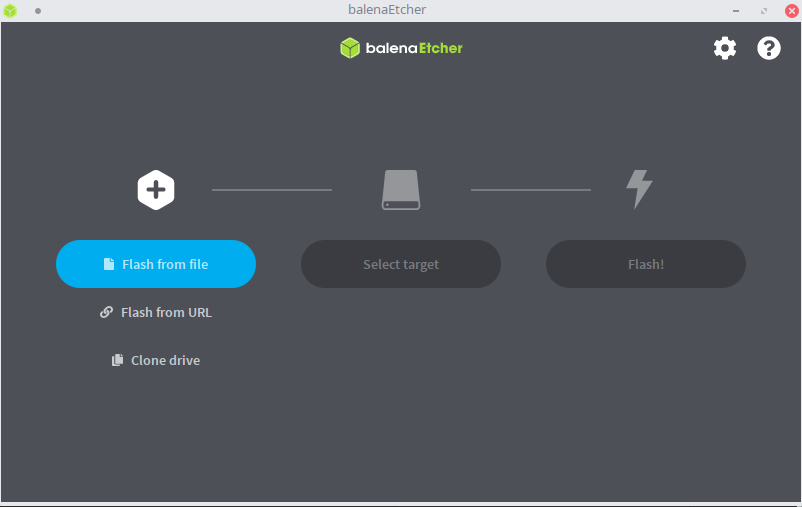
\includegraphics[width=0.7\textwidth]{image/image-20231015121217662.png}
  \caption{BalenaEtcher界面}
\end{figure}


\subsection{ssh连接visionfive 2}

通过HDMI使用Xfce桌面环境登录, 用户名和密码如下:
\begin{enumerate}
\item Username: root
\item Password: starfive
\end{enumerate}

然后需要设置允许root用户通过ssh登录,通过使用以下命令进行修改:
\begin{lstlisting}
  echo "PermitRootLogin yes" >> /etc/ssh/sshd_config
\end{lstlisting}

修改完成后,使用以下命令进行重启ssh服务器:
\begin{lstlisting}
  /etc/init.d/ssh restart
\end{lstlisting}

使用浏览器登录到路由器地址,找到昉·星光 2的IP地址之后,通过ssh登录开发版,如下:

\begin{lstlisting}
  ssh root@192.168.1.xxx
\end{lstlisting}

完成此步后,需要输入密码才能完成登录。接下来到步骤需要使用gcc和vim,通过使用以下到命令进行安装gcc和vim:

\begin{lstlisting}
apt update
apt install gcc vim  
\end{lstlisting}

\section{反编译c语言代码}
安装好gcc和vim后,现在可以进行本次实验到核心操作——“反编译c语言代码”。首先使用vim创建main.c文件,使用下列的命令即可完成创建:
\begin{lstlisting}
  vim main.c  
\end{lstlisting}

将下列到示例代码复制以下代码到main.c,需要注意的是在使用vim打开main.c后,vim此时处于不可编辑到状态,需要轻点一次“i”键才能使用粘贴键。示例代码如下:

\begin{lstlisting}
// main.c
int g(int x)
{
    return x + 3;
}
    
int f(int x)
{
    return g(x);
}
    
int main(void)
{
    return f(8) + 1;
}  
\end{lstlisting}

完成好编辑任务后,使用以下的命令让gcc进行编译,使得c语言编译成为RISCV架构下汇编语言。命令如下:

\begin{lstlisting}
  gcc -S -o main.s main.c
\end{lstlisting}

得到\lstinline{main.S}后,使用vim打开,内容如下:
\begin{lstlisting}
	.file	"main.c"
	.option pic
	.text
	.align	1														
	.globl	g
	.type	g, @function
g:
	addi	sp,sp,-32
	sd	s0,24(sp)
	addi	s0,sp,32
	mv	a5,a0
	sw	a5,-20(s0)
	lw	a5,-20(s0)
	addiw	a5,a5,3
	sext.w	a5,a5
	mv	a0,a5
	ld	s0,24(sp)
	addi	sp,sp,32
	jr	ra
	.size	g, .-g
	.align	1
	.globl	f
	.type	f, @function
f:
	addi	sp,sp,-32
	sd	ra,24(sp)
	sd	s0,16(sp)
	addi	s0,sp,32
	mv	a5,a0
	sw	a5,-20(s0)
	lw	a5,-20(s0)
	mv	a0,a5
	call	g
	mv	a5,a0
	mv	a0,a5
	ld	ra,24(sp)
	ld	s0,16(sp)
	addi	sp,sp,32
	jr	ra
	.size	f, .-f
	.align	1
	.globl	main
	.type	main, @function
main:
	addi	sp,sp,-16
	sd	ra,8(sp)
	sd	s0,0(sp)
	addi	s0,sp,16
	li	a0,8
	call	f
	mv	a5,a0
	addiw	a5,a5,1
	sext.w	a5,a5
	mv	a0,a5
	ld	ra,8(sp)
	ld	s0,0(sp)
	addi	sp,sp,16
	jr	ra
	.size	main, .-main
	.ident	"GCC: (Debian 11.3.0-3) 11.3.0"
	.section	.note.GNU-stack,"",@progbits

\end{lstlisting}

在vim的命令模式下,使用\lstinline{ :g/.*./d}正则表达式删除带有的. 的行

\begin{lstlisting}
g:
	addi	sp,sp,-32
	sd	s0,24(sp)
	addi	s0,sp,32
	mv	a5,a0
	sw	a5,-20(s0)
	lw	a5,-20(s0)
	addiw	a5,a5,3
	mv	a0,a5
	ld	s0,24(sp)
	addi	sp,sp,32
	jr	ra
f:
	addi	sp,sp,-32
	sd	ra,24(sp)
	sd	s0,16(sp)
	addi	s0,sp,32
	mv	a5,a0
	sw	a5,-20(s0)
	lw	a5,-20(s0)
	mv	a0,a5
	call	g
	mv	a5,a0
	mv	a0,a5
	ld	ra,24(sp)
	ld	s0,16(sp)
	addi	sp,sp,32
	jr	ra
main:
	addi	sp,sp,-16
	sd	ra,8(sp)
	sd	s0,0(sp)
	addi	s0,sp,16
	li	a0,8
	call	f
	mv	a5,a0
	addiw	a5,a5,1
	mv	a0,a5
	ld	ra,8(sp)
	ld	s0,0(sp)
	addi	sp,sp,16
	jr	ra
\end{lstlisting}
实验一到此结束。

\chapter{实验二:完成一个简单的时间片轮转多道程序内核代码}
\section{串口连接开发板}
我们使用USB转TTY下载线连接Starfive旗下的VisionFive2开发板。主机操作系统是Ubuntu22.04,具体配置如下。


\begin{figure}[htbp]
  \centering
  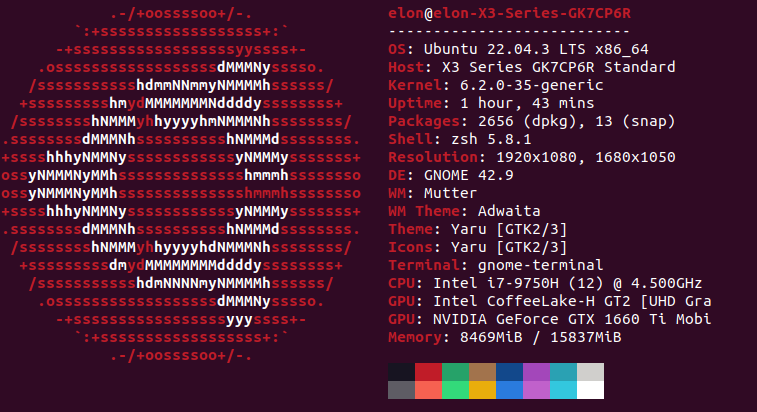
\includegraphics[width=0.7\textwidth]{image/image-20231029115426545.png}
  \caption{系统配置}
\end{figure}


引脚连接实物图如下:

\begin{figure}[htbp]
  \centering
  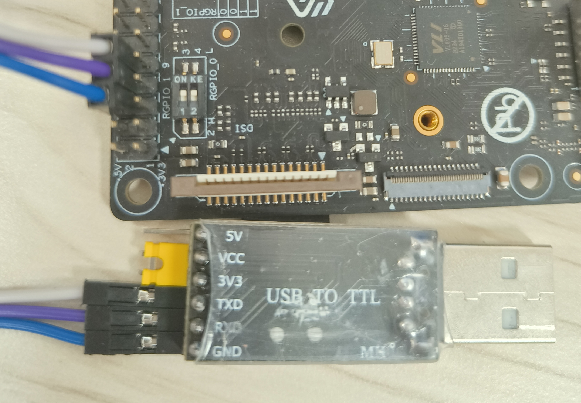
\includegraphics[width=0.7\textwidth]{image/image-20231029115801584.png}
  \caption{引脚连接实物图}
\end{figure}

\newpage
\section{mincom串口工具下载与设置}

使用以下命令进行下载串口工具下载:
\begin{lstlisting}
    sudo apt update
    sudo apt install minicom
\end{lstlisting}

使用以下命令对串口工具进行设置:
\begin{lstlisting}
  sudo minicom -s  
\end{lstlisting}

进入minicom的设置界面后:方向键选择 Serial port setup后按回车确定。

\begin{figure}[htbp]
  \centering
  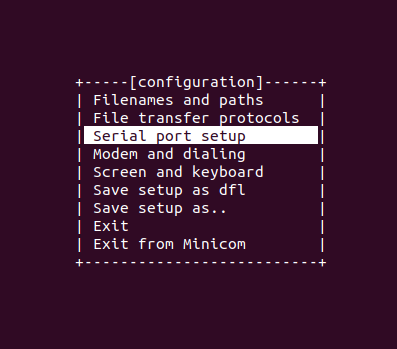
\includegraphics[width=0.3\textwidth]{image/image-20231029120122847.png}
  \caption{minicom设置界面1}
\end{figure}

进入串口设置界面后:按Shift+a选择Serial Device,将设备名改为/dev/ttyUSB0.

\begin{figure}[htbp]
  \centering
  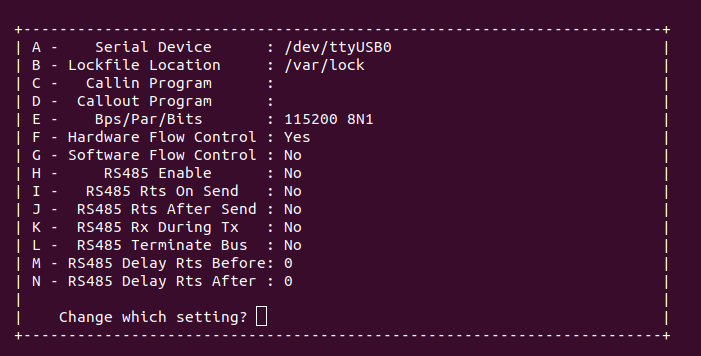
\includegraphics[width=0.5\textwidth]{image/image-20231029120332044.png}
  \caption{minicom设置界面2}
\end{figure}

修改完成后按下回车,返回上级菜单后,选择Save setup as dfl保存配置。

\begin{figure}[htbp]
  \centering
  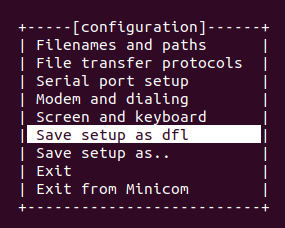
\includegraphics[width=0.3\textwidth]{image/image-20231029120447877.png}
  \caption{minicom设置界面3}
\end{figure}

保存后,选择Exit退出Minicom

使用Minicom连接VisionFive2
首先将连接好引脚的USB插口插入笔记本上,然后使用以下命令启动Minicom。

\begin{lstlisting}
  sudo minicom  
\end{lstlisting}

如果启动失败显示没有/dev/ttyUSB0,请参见下一节《CH340系列串口驱动占用》。

启动后会显示进入minicom。然后使用电源线连接开发板,给开发板加电。此时Minicom会开始显示加电后各种程序启动的信息:

\begin{figure}[htbp]
  \centering
  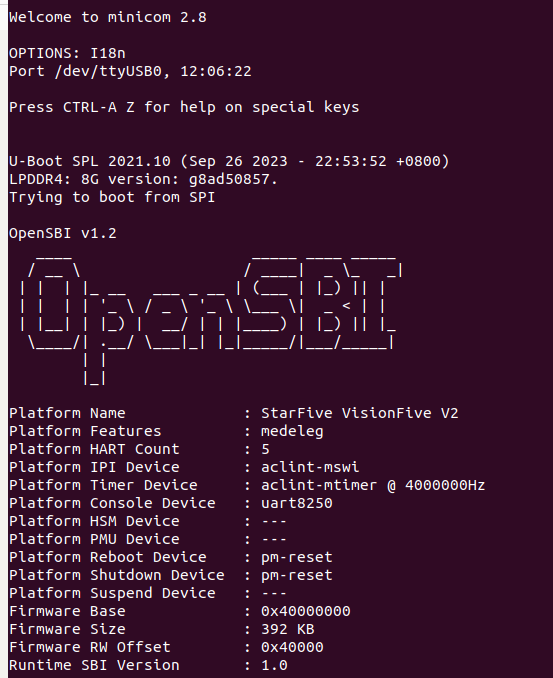
\includegraphics[width=0.5\textwidth]{image/image-20231029121051751.png}
  \caption{minicom启动}
\end{figure}

\section{CH340系列串口驱动占用}
如果配置好Minicom后显示没有ttyUSB的问题,那么可能是由于CH340系列串口驱动被占用。

使用以下命令判断是否驱动被占用:
\begin{lstlisting}
  sudo dmesg | grep brltty
\end{lstlisting}
如果显示以下信息:

\begin{lstlisting}
  [ 7033.078452] usb 1-13: usbfs: interface 0 claimed by ch341 while &apos;brltty&apos; sets config #1
\end{lstlisting}

说明:驱动占用

解决方法:使用以下命令卸载brltty

\begin{lstlisting}
  sudo apt remove brltty
\end{lstlisting}

然后重新进行插拔USB接口,并使用以下的命令查看是否恢复正常:

\begin{lstlisting}
  ls /dev/ttyUSB0 
\end{lstlisting}
若显示:

\begin{lstlisting}
  ls /dev/ttyUSB0 
  /dev/ttyUSB0
\end{lstlisting}
说明恢复正常,可以按照之前的步骤继续实验。

\section{为编译Linux内核做准备}

StarFive为VisionFive2提供了一个GitHub仓库,阅读这个仓库中的README文件是本次实验的一部分。从README得知,为连编译能够在开发板上运行的Linux内核,首先需要为编译提供依赖环境。

使用以下的命令,在ubuntu22.04上创建可实现交叉编译risc-v架构的环境依赖:

\begin{lstlisting}
  sudo apt update
  sudo apt-get install build-essential automake libtool texinfo bison flex gawk g++ git xxd curl wget gdisk gperf cpio bc screen texinfo unzip libgmp-dev libmpfr-dev libmpc-dev libssl-dev libncurses-dev libglib2.0-dev libpixman-1-dev libyaml-dev patchutils python3-pip zlib1g-dev device-tree-compiler dosfstools mtools kpartx rsync
\end{lstlisting}
安装Git LFS:

\begin{lstlisting}
  curl -s https://packagecloud.io/install/repositories/github/git-lfs/script.deb.sh | sudo bash
  sudo apt-get install git-lfs
\end{lstlisting}

需要注意的是安装Git LFS需要访问外网,要完成此步骤需读者自行解决访问外网的问题或者使用国内镜像网站。

克隆VisionFive2 仓库
使用以下命令克隆VisionFive2:

\begin{lstlisting}
git clone https://github.com/starfive-tech/VisionFive2.git
cd VisionFive2
git checkout JH7110_VisionFive2_devel
git submodule update --init --recursive
\end{lstlisting}

切换分支:

\begin{lstlisting}
cd buildroot && git checkout --track origin/JH7110_VisionFive2_devel && cd ..
cd u-boot && git checkout --track origin/JH7110_VisionFive2_devel && cd ..
cd linux && git checkout --track origin/JH7110_VisionFive2_devel && cd ..
cd opensbi && git checkout master && cd ..
cd soft_3rdpart && git checkout JH7110_VisionFive2_devel && cd ..
\end{lstlisting}

\section{RISC-V架构MyKernel内核的构建}
\subsection{实验目的和实验内容}
这次实验主要目的是初识RISC—V架构。简单的了解一下RISC-V下的汇编,理解代码在RISC-V下是怎么跑起来的。
我们将会实现一个非常简单的进程调度器,来帮助我们理解操作系统和RISC-V。

\subsection{了解riscv}
如果需要更加详细的了解请参考:

\begin{itemize}
  \item \href{http://riscvbook.com/chinese/RISC-V-Reader-Chinese-v2p1.pdf}{RISC-V中文参考}
  \item The RISC-V Instruction Set Manual(\href{https://github.com/riscv/riscv-isa-manual/releases/download/Priv-v1.12/riscv-privileged-20211203.pdf}{Volume I} , \href{https://github.com/riscv/riscv-isa-manual/releases/download/Ratified-IMAFDQC/riscv-spec-20191213.pdf}{Volume II})
  \item \href{https://github.com/riscv-non-isa/riscv-elf-psabi-doc}{ABI for RISC-V}
\end{itemize}

我们这里只是简单的了解一下riscv寄存器的 RISC-V 应用程序二进制接口(ABI)

\begin{figure}[htbp]
  \centering
  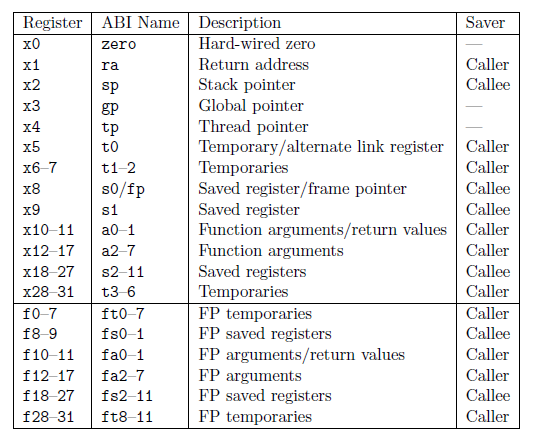
\includegraphics[width=0.7\textwidth]{image/regfile.png}
  \caption{RISCV 寄存器}
\end{figure}

这些寄存器是riscv的通用寄存器,一共有32个,在这一章我们可能会用到ra寄存器:保存函数返回地址。sp寄存器:保存函数的栈指针。

函数是怎么执行的
我们都知道,c语言会被转化成汇编在转化成机器码。而汇编和机器码之间的转换是直接转换的。所以我们理解了一个函数在汇编上怎么运行的,那么我们就能理解函数在计算机上是如何运行的。

\say{我们这里使用的是RISC-V的指令架构,所以我们只讲解RISC-V下的汇编代码。但是为了更好的理解,我强烈建议先阅读理解x86下函数是怎么运行的。

\begin{itemize}
  \item \href{https://www.cnblogs.com/clover-toeic/p/3755401.html}{C语言函数调用栈(一)}
  \item \href{https://www.cnblogs.com/clover-toeic/p/3756668.html}{C语言函数调用栈(二)}
\end{itemize}
}


首先我们来看在初入计算机世界的时候,我们遇到的第一份代码hello world的反汇编代码。

\begin{lstlisting}
  #include <stdiio.h>
  int main(){
    printf("hello world");
  }
\end{lstlisting}

我们编译好之后用objdump反汇编一下,我这里去除掉了一些不需要的信息,只保留main函数的部分。
\begin{lstlisting}
  hello:     file format elf64-littleriscv

  Disassembly of section .text:
  
  000000000000062a <main>:
  62a:   1141                    addi    sp,sp,-16
  62c:   e406                    sd      ra,8(sp)
  62e:   e022                    sd      s0,0(sp)
  630:   0800                    addi    s0,sp,16
  632:   00000517                auipc   a0,0x0
  636:   07650513                addi    a0,a0,118 # 6a8 <__libc_csu_fini+0x6>
  63a:   f17ff0ef                jal     ra,550 <printf@plt>
  63e:   4781                    li      a5,0
  640:   853e                    mv      a0,a5
  642:   60a2                    ld      ra,8(sp)
  644:   6402                    ld      s0,0(sp)
  646:   0141                    addi    sp,sp,16
  648:   8082                    ret
\end{lstlisting}

我们来分析一下这段代码:

首先addi sp,sp,-16的作用是开栈(这里假定对函数栈有一定的了解,如果不了解请阅读上文的c语言函数调用栈 ),为函数开辟自己的栈帧。

然后是sd ra,8(sp)和sd s0,0(sp) 这是将ra和s0分别存储在sp+8和sp+0的位置。这个里这个ra是函数的返回地址(调用者调用此函数的下一条指令)当函数执行完后,此函数的调用者时就是跳转到ra中存储的位置,如果此函数时最末端的叶子调用,是不用将其存入栈里面的。s0是函数的栈的栈底,也就是帧指针。
接下来是函数内部的一些计算跳转,我们先不管。

直接看到下面的642位置 ld ra,8(sp)和644ld s0.0(sp) 这两个指令是把函数在开始存储的返回地址和帧指针重新加载进相应的寄存器

然后是addi sp,sp,-16收回栈帧。 最后ret,这个ret是个伪指令,实际上是jar ra

那么我们就可以大概了解函数是怎么运行的了:
\begin{enumerate}
\item 首先为函数开辟栈帧
\item 接着存储返回地址和上个栈帧的基址
\item 运算
\item 将存储的返回地址和帧地址重新加载进相应的寄存器
\item 收回栈帧
\item 返回上个函数调用此函数的位置的下一条指令。
\end{enumerate}


\subsection{制作我们的简易调度器}
有了以上信息后,理论上我们已经可以手写汇编了,那么我们来完成一下我们的内容:编写一个简单的调度器。
首先制定我们的需求:
\begin{itemize}
  \item 可以进行进程切换
  \item 简单
\end{itemize}

那么一个进程里面会有什么呢--pc寄存器加上通用寄存器,加上函数的栈帧。我们一般称之为函数现场。当现场没变,那么程序的状态就没变。也就是说当我们保存了现场,然后切换到其他进程运行一段时间后,恢复它那么我们就能切换回来,继续运行。那么我们就可以定义一个时间片段,允许每个进程运行一段时间然后切换到其他进程。这样我们就能做到根据时间片的多个进程的轮转调度了。

但是riscv的通用寄存器有32个,很多,我们其实是不需要全部保存的,只需要保存caller save的寄存器。但是对此时的我们来说还是有点多,我们可以再精简一点,省去我们不需要的寄存器,比如有关浮点数的寄存器我们这里是用不到的。

首先我们得有一个存储现场的地方,我们将现场存储在pcb的AThread里面,每次切换出去的时候把它保存进来,切换回来的时候,从这里把寄存器重新加载进去。

注意这里的\_\_switch函数,在这里我们写了两部分的汇编代码。第一部分就是是将当前的各种寄存器存入内存,第二部分就是将内存中存储的值加载进寄存器。但是函数入口会改变栈,所以在存储之前我们先要将函数入口给回退。

这部分的代码逻辑就很清晰了,定时器中断里面的值达到我们期望的值的时候进行一次进程切换。

\begin{lstlisting}
//mypcb.h

/*
 *  linux/mykernel/mypcb.h
 *
 *  Kernel internal PCB types
 *
 *  Copyright (C) 2023  WangRui
 *
 */

#define MAX_TASK_NUM        4
#define KERNEL_STACK_SIZE   1024*2
/* CPU-specific state of this task */
//初始状态
typedef struct Thread {
    unsigned long       s0;
    unsigned long		ip;
    unsigned long		sp;
}tThread;
//保存的现场
typedef struct AThread {
    //unsigned long       s0;
    unsigned long		ra;
    unsigned long		sp;
    unsigned long		s0;
    unsigned long		s1;
    unsigned long		s2;
    unsigned long		s3;
    unsigned long		s4;
    unsigned long		s5;
    unsigned long		s6;
    unsigned long		s7;
    unsigned long		s8;
    unsigned long		s9;
    unsigned long		s10;
    unsigned long		s11;
}aThread;

typedef struct PCB{
    int pid;
    volatile long state;	/* -1 unrunnable, 0 runnable, >0 stopped */
	unsigned long stack[KERNEL_STACK_SIZE];//在这里存储进程的整个栈。
    /* CPU-specific state of this task */
    struct Thread thread;
    unsigned long	task_entry;
    struct PCB *next;	
}tPCB;

void my_schedule(void);

\end{lstlisting}

这部分代码主要是一些数据结构的定义,我们把一个进程的状态抽象成一个pcb块,在这里我们存入最主要的几个数据:

\begin{itemize}
  \item pid:进程的进程号,是一个标识符,它是唯一的。
  \item state: 用来表示进程当前的状态。如果是runnaable的话就可以被进程调度器发现,并且参与调度。
  \item stack: 程序运行时所使用的栈空间,每个程序的栈空间时不一样的。
  \item thread:用来保存程序运行时的寄存器状态,即现场。
  \item tash\_entry: 用来表示程序的入口地址,简单理解相当于我们平时编程的main函数。
  \item next: 表示下一个程序的地址。
\end{itemize}


\begin{lstlisting}
// my_schdule
/*
 *  linux/mykernel/myinterrupt.c
 *
 *  Kernel internal my_timer_handler
 *
 *  Copyright (C) 2023, 2023  WangRui
 *
 */
#include <linux/types.h>
#include <linux/string.h>
#include <linux/ctype.h>
#include <linux/tty.h>
#include <linux/vmalloc.h>

#include "mypcb.h"

extern tPCB task[MAX_TASK_NUM];
extern tPCB * my_current_task;
extern volatile int my_need_sched;
volatile int time_count = 0;

/*
 * Called by timer interrupt.
 * it runs in the name of current running process,
 * so it use kernel stack of current running process
 */
//我们的定时器

void my_timer_handler(void)
{
    if(time_count%1000 == 0 && my_need_sched != 1)
    {
        printk(KERN_NOTICE ">>>my_timer_handler here<<<\n");
        my_need_sched = 1;
    } 
    time_count ++ ;  
    return;  	
}

void __switch(aThread * old,aThread *new){
    //old a0 new a1
    asm volatile (
        "add s0,sp,-16\n"
        "ld s0,8(sp)\n"
        "add sp,sp,16\n"
        "sd ra,0(%[old]) \n"
        "sd sp,8(%[old]) \n"
        "sd s0,16(%[old]) \n"
        "sd s1,24(%[old]) \n"
        "sd s2,32(%[old]) \n"
        "sd s3,40(%[old]) \n"
        "sd s4,48(%[old]) \n"
        "sd s5,56(%[old]) \n"
        "sd s6,64(%[old]) \n"
        "sd s7,72(%[old]) \n"
        "sd s8,80(%[old]) \n"
        "sd s9,88(%[old]) \n"
        "sd s10,96(%[old]) \n"
        "sd s11,104(%[old]) \n"
        

        "ld ra, 0(%[new]) \n"
        "ld sp, 8(%[new]) \n"
        "ld s0, 16(%[new]) \n"
        "ld s1, 24(%[new]) \n"
        "ld s2, 32(%[new]) \n"
        "ld s3, 40(%[new]) \n"
        "ld s4, 48(%[new]) \n"
        "ld s5, 56(%[new]) \n"
        "ld s6, 64(%[new]) \n"
        "ld s7, 72(%[new]) \n"
        "ld s8, 80(%[new]) \n"
        "ld s9, 88(%[new]) \n"
        "ld s10, 96(%[new]) \n"
        "ld s11, 104(%[new]) \n"
        "ret \n"
        : 
        : [old] "r" (old),[new] "r" (new)
    );
}
//调度器
void my_schedule(void)
{
    tPCB * next;
    tPCB * prev;

    if(my_current_task == 0
        || my_current_task->next == 0)
    {
    	return;
    }
    print(">>>my_schedule<<<\n");
    /* schedule */
    next = my_current_task->next;
    prev = my_current_task;
    if(next->state == 0)/* -1 unrunnable, 0 runnable, >0 stopped */
    {        
    	my_current_task = next;
        print("stacks : %p\n",task->context.sp); 
    	print(">>>switch %d to %d<<<\n",prev->pid,next->pid);  
        __switch(&prev->context, &next->context);
        print("after scheduler\n"); 
    }  
    return;	
}

\end{lstlisting}
这里的my\_time\_handler函数时一个定时器中断所调用的函数,每当计算机产生一次定时器中断,就会调用这个函数。这个函数的作用是当触发了一定的定时器中断之后,就开启调度器。有了这个我们就能让我们的程序按时间片进行轮转运行了。
而这里的my\_schdule就是我们的调度器,他最主要的是\_\_switch函数这个函数会将此时运行的程序的寄存器保存进prev结构体里面,然后将下一个进程的寄存器状态从next结构体里面取出来,并且加载进寄存器。

\begin{lstlisting}
// 初始化
/*
 *  linux/mykernel/mymain.c
 *
 *  Kernel internal my_timer_handler
 *
 *  Copyright (C) 2023, 2023  WangRui
 *  
 */
#include <linux/types.h>
#include <linux/string.h>
#include <linux/ctype.h>
#include <linux/tty.h>
#include <linux/vmalloc.h>


#include "mypcb.h"

tPCB task[MAX_TASK_NUM];
tPCB * my_current_task = NULL;
volatile int my_need_sched = 0;

void my_process(void);


void __init_my_start_kernel(void)
{

    print("run init my start kernel");
    int pid = 0;
    int i;
    /* Initialize process 0*/
    //unsigned long stacks = 0xffffffff81601000;
    
    task[pid].pid = pid;
    task[pid].state = 0;/* -1 unrunnable, 0 runnable, >0 stopped */
    task[pid].task_entry = task[pid].thread.ip = (unsigned long)my_process;
    task[pid].thread.sp = (unsigned long)&task[pid].stack[KERNEL_STACK_SIZE-1];
    task[pid].thread.s0 = (unsigned long)&task[pid].stack[KERNEL_STACK_SIZE-1];
    task[pid].next = &task[pid];   

    task[pid].context.ra = (unsigned long)my_process;
    task[pid].context.s0 = (unsigned long)&task[pid].stack[KERNEL_STACK_SIZE-1];
    task[pid].context.sp = (unsigned long)&task[pid].stack[KERNEL_STACK_SIZE-1];
    
    /*fork more process */
    for(i=1;i<MAX_TASK_NUM;i++)
    {
        memcpy(&task[i],&task[0],sizeof(tPCB));
        task[i].pid = i;
	    task[i].thread.sp = (unsigned long)(&task[i].stack[KERNEL_STACK_SIZE-1]);
        
        task[i].context.s0 = (unsigned long)&task[i].stack[KERNEL_STACK_SIZE-1];
        task[i].context.sp = (unsigned long)&task[i].stack[KERNEL_STACK_SIZE-1];
        
        task[i].next = task[i-1].next;
        task[i-1].next = &task[i];
    }
    print("stacks : %p\n",task[0].thread.sp);
    /* start process 0 by task[0] */
    pid = 0;
    my_current_task = &task[pid];
	__asm__ volatile(
        "mv sp,%[msp]\n"
        "mv ra,%[mip]\n"
        "mv s0,%[ms0]\n"
    	"ret\n\t" 	            /* pop task[pid].thread.ip to rip */
    	: 
    	:[mip] "r" (task[pid].thread.ip),[msp] "r" (task[pid].thread.sp), [ms0]"r" (task[pid].thread.s0)	/* input c or d mean %ecx/%edx*/
	);
} 

int i = 0;

void my_process(void)
{    
    while(1)
    {
        i++;
        if(i%10000000 == 0)
        {
            printk(KERN_NOTICE "this is process %d -\n",my_current_task->pid);
            if(my_need_sched == 1)
            {
                my_need_sched = 0;
        	    my_schedule();
        	}
        	printk(KERN_NOTICE "this is process %d +\n",my_current_task->pid);
        }     
    }
}

\end{lstlisting}

这里的my\_kernel\_start函数主要是进行一些初始化,其实主要就是初始化进程运行的栈空间,和entry的地址,这里的汇编代码的作用是将第一个程序的entry地址填入ra之中,而我们都知道ra是保存的是函数返回之后,下一条指令运行的地址,所以我们在这里将entry直接加载进ra然后跳转到这个地址,这样我们就能改变函数的运行顺序,从而进入我们自己写的程序里面。

Makefile:

\begin{lstlisting}
obj-y     = mymain.o myinterrupt.o
kernel.patch:

diff --color -Naru Linux/drivers/clocksource/timer-riscv.c linux/drivers/clocksource/timer-riscv.c
--- Linux/drivers/clocksource/timer-riscv.c	2023-10-25 19:29:12.000000000 +0800
+++ linux/drivers/clocksource/timer-riscv.c	2023-10-29 16:10:34.294399984 +0800
@@ -20,6 +20,8 @@
 #include <asm/smp.h>
 #include <asm/sbi.h>
 #include <asm/timex.h>
+//change
+#include "linux/timer.h"

 static int riscv_clock_next_event(unsigned long delta,
 		struct clock_event_device *ce)
@@ -86,7 +88,7 @@

 	csr_clear(CSR_IE, IE_TIE);
 	evdev->event_handler(evdev);
-
+	my_timer_handler();
 	return IRQ_HANDLED;
 }

diff --color -Naru Linux/include/linux/start_kernel.h linux/include/linux/start_kernel.h
--- Linux/include/linux/start_kernel.h	2023-10-25 19:29:16.000000000 +0800
+++ linux/include/linux/start_kernel.h	2023-10-29 16:16:36.018535237 +0800
@@ -7,7 +7,8 @@

 /* Define the prototype for start_kernel here, rather than cluttering
    up something else. */
-
+//change
+extern void __init my_start_kernel(void);
 extern asmlinkage void __init start_kernel(void);
 extern void __init arch_call_rest_init(void);
 extern void __ref rest_init(void);
diff --color -Naru Linux/include/linux/timer.h linux/include/linux/timer.h
--- Linux/include/linux/timer.h	2023-10-25 19:29:16.000000000 +0800
+++ linux/include/linux/timer.h	2023-10-29 16:19:31.419156143 +0800
@@ -191,7 +191,8 @@
 #endif

 #define del_singleshot_timer_sync(t) del_timer_sync(t)
-
+//change
+extern void my_timer_handler(void);
 extern void init_timers(void);
 struct hrtimer;
 extern enum hrtimer_restart it_real_fn(struct hrtimer *);
diff --color -Naru Linux/init/main.c linux/init/main.c
--- Linux/init/main.c	2023-10-25 19:29:16.000000000 +0800
+++ linux/init/main.c	2023-10-29 16:22:14.563230772 +0800
@@ -1137,7 +1137,8 @@
 	acpi_subsystem_init();
 	arch_post_acpi_subsys_init();
 	kcsan_init();
-
+	//change
+	my_start_kernel();
 	/* Do the rest non-__init'ed, we're now alive */
 	arch_call_rest_init();

diff --color -Naru Linux/Makefile linux/Makefile
--- Linux/Makefile	2023-10-25 19:29:11.000000000 +0800
+++ linux/Makefile	2023-10-29 16:24:49.013860022 +0800
@@ -1115,7 +1115,9 @@
 export MODULES_NSDEPS := $(extmod_prefix)modules.nsdeps

 ifeq ($(KBUILD_EXTMOD),)
-core-y		+= kernel/ certs/ mm/ fs/ ipc/ security/ crypto/ block/
+#core-y		+= kernel/ certs/ mm/ fs/ ipc/ security/ crypto/ block/
+#change
+core-y		+= kernel/ certs/ mm/ fs/ ipc/ security/ crypto/ block/ mykernel/

 vmlinux-dirs	:= $(patsubst %/,%,$(filter %/, \
 		     $(core-y) $(core-m) $(drivers-y) $(drivers-m) \
diff --color -Naru Linux/mykernel/Makefile linux/mykernel/Makefile
--- Linux/mykernel/Makefile	1970-01-01 08:00:00.000000000 +0800
+++ linux/mykernel/Makefile	2023-10-29 16:05:02.543702121 +0800
@@ -0,0 +1 @@
+obj-y     = mymain.o myinterrupt.o
diff --color -Naru Linux/mykernel/myinterrupt.c linux/mykernel/myinterrupt.c
--- Linux/mykernel/myinterrupt.c	1970-01-01 08:00:00.000000000 +0800
+++ linux/mykernel/myinterrupt.c	2023-10-29 17:58:31.532334640 +0800
@@ -0,0 +1,86 @@
+/*
+ *  linux/mykernel/myinterrupt.c
+ *
+ *  Kernel internal my_timer_handler
+ *  Change IA32 to x86-64 arch, 2020/4/26
+ *
+ *  Copyright (C) 2013, 2020  Mengning
+ *
+ */
+#include <linux/types.h>
+#include <linux/string.h>
+#include <linux/ctype.h>
+#include <linux/tty.h>
+#include <linux/vmalloc.h>
+
+#include "mypcb.h"
+
+extern tPCB task[MAX_TASK_NUM];
+extern tPCB * my_current_task;
+extern volatile int my_need_sched;
+volatile int time_count = 0;
+
+/*
+ * Called by timer interrupt.
+ * it runs in the name of current running process,
+ * so it use kernel stack of current running process
+ */
+void my_timer_handler(void)
+{
+    if(time_count%1000 == 0 && my_need_sched != 1)
+    {
+        printk(KERN_NOTICE ">>>my_timer_handler here<<<\n");
+        my_need_sched = 1;
+    }
+    time_count ++ ;
+    return;  	
+}
+
+void my_schedule(void)
+{
+    tPCB * next;
+    tPCB * prev;
+
+    if(my_current_task == NULL
+        || my_current_task->next == NULL)
+    {
+    	return;
+    }
+    printk(KERN_NOTICE ">>>my_schedule<<<\n");
+    /* schedule */
+    next = my_current_task->next;
+    prev = my_current_task;
+    if(next->state == 0)/* -1 unrunnable, 0 runnable, >0 stopped */
+    {
+    	my_current_task = next;
+        unsigned long prev_sp = prev->thread.sp;
+        unsigned long prev_ra = next->thread.ra;
+    	unsigned long next_sp = next->thread.sp;
+        unsigned long next_ra = next->thread.ra;
+    	printk(KERN_NOTICE ">>>switch %d to %d<<<\n",prev->pid,next->pid);
+    	/* switch to next process */
+    	// __asm__ volatile(	
+        //     "mv %0,sp \n"
+        //     "mv %1,ra \n"
+        //     "ld sp,%2 \n"
+        //     "ld ra,%3 \n"
+        //     "ret"
+        // 	: "=r" (prev->thread.sp),"=r" (prev->thread.ra)
+        // 	: "m" (next->thread.sp), "m" ( next->thread.ra)
+    	// );
+        __asm__ volatile (
+            "mv %0,sp \n"
+            "mv %1,ra \n"
+            :"=r" (prev_sp) ,"=r" (prev_ra)
+        );
+        __asm__ volatile(	
+
+            "mv sp,%0 \n"
+            "mv ra,%1 \n"
+            "ret"
+        	:
+            : "r" (next_sp), "r" ( next_ra)
+    	);
+    }
+    return;	
+}
diff --color -Naru Linux/mykernel/mymain.c linux/mykernel/mymain.c
--- Linux/mykernel/mymain.c	1970-01-01 08:00:00.000000000 +0800
+++ linux/mykernel/mymain.c	2023-10-29 14:51:20.000000000 +0800
@@ -0,0 +1,75 @@
+/*
+ *  linux/mykernel/mymain.c
+ *
+ *  Kernel internal my_start_kernel
+ *  Change IA32 to x86-64 arch, 2020/4/26
+ *
+ *  Copyright (C) 2013, 2020  Mengning
+ *
+ */
+#include <linux/types.h>
+#include <linux/string.h>
+#include <linux/ctype.h>
+#include <linux/tty.h>
+#include <linux/vmalloc.h>
+
+
+#include "mypcb.h"
+
+tPCB task[MAX_TASK_NUM];
+tPCB * my_current_task = NULL;
+volatile int my_need_sched = 0;
+
+void my_process(void);
+
+
+void __init my_start_kernel(void)
+{
+    int pid = 0;
+    int i;
+    /* Initialize process 0*/
+    task[pid].pid = pid;
+    task[pid].state = 0;/* -1 unrunnable, 0 runnable, >0 stopped */
+    task[pid].task_entry = task[pid].thread.ra = (unsigned long)my_process;
+    task[pid].thread.sp = (unsigned long)&task[pid].stack[KERNEL_STACK_SIZE-1];
+    task[pid].next = &task[pid];
+    /*fork more process */
+    for(i=1;i<MAX_TASK_NUM;i++)
+    {
+        memcpy(&task[i],&task[0],sizeof(tPCB));
+        task[i].pid = i;
+	    task[i].thread.sp = (unsigned long)(&task[i].stack[KERNEL_STACK_SIZE-1]);
+        task[i].next = task[i-1].next;
+        task[i-1].next = &task[i];
+    }
+    /* start process 0 by task[0] */
+    pid = 0;
+    my_current_task = &task[pid];
+	__asm__ volatile(
+        "mv sp,%[sp]\n"
+        "mv ra,%[ra]\n"
+        "ret"
+    	:
+    	: [ra] "r" (task[pid].thread.ra),[sp] "r" (task[pid].thread.sp)	/* input c or d mean %ecx/%edx*/
+	);
+}
+
+int i = 0;
+
+void my_process(void)
+{
+    while(1)
+    {
+        i++;
+        if(i%10000000 == 0)
+        {
+            printk(KERN_NOTICE "this is process %d -\n",my_current_task->pid);
+            if(my_need_sched == 1)
+            {
+                my_need_sched = 0;
+        	    my_schedule();
+        	}
+        	printk(KERN_NOTICE "this is process %d +\n",my_current_task->pid);
+        }
+    }
+}
diff --color -Naru Linux/mykernel/mypcb.h linux/mykernel/mypcb.h
--- Linux/mykernel/mypcb.h	1970-01-01 08:00:00.000000000 +0800
+++ linux/mykernel/mypcb.h	2023-10-29 14:51:27.000000000 +0800
@@ -0,0 +1,29 @@
+/*
+ *  linux/mykernel/mypcb.h
+ *
+ *  Kernel internal PCB types
+ *
+ *  Copyright (C) 2013  Mengning
+ *
+ */
+
+#define MAX_TASK_NUM        4
+#define KERNEL_STACK_SIZE   1024*2
+/* CPU-specific state of this task */
+struct Thread {
+    unsigned long		ra;
+    unsigned long		sp;
+};
+
+typedef struct PCB{
+    int pid;
+    volatile long state;	/* -1 unrunnable, 0 runnable, >0 stopped */
+    unsigned long stack[KERNEL_STACK_SIZE];
+    /* CPU-specific state of this task */
+    struct Thread thread;
+    unsigned long	task_entry;
+    struct PCB *next;
+}tPCB;
+
+void my_schedule(void);
+
\end{lstlisting}

使用以下到命令进行补丁打包:
\begin{lstlisting}
  patch -p1 < ../kernel.patch  
\end{lstlisting}

\section{编译RISC-V架构MyKernel内核}
将上一节生成的linux内核目录替换VisionFive2中的linux内核目录后,使用以下命令进行编译。

\begin{lstlisting}
  make -j$(nproc)
\end{lstlisting}

此次编译时间较长,编译成功后会在VisionFive2中自动创建work目录,所有的编译完成的文件都会在这个目录中生成。成功编译后,文件结构如图所示:

\begin{lstlisting}
  work/
  ├── visionfive2_fw_payload.img
  ├── image.fit
  ├── initramfs.cpio.gz
  ├── u-boot-spl.bin.normal.out
  ├── linux/arch/riscv/boot
  ├── dts
  │   └── starfive
  │       ├── jh7110-visionfive-v2-ac108.dtb
  │       ├── jh7110-visionfive-v2.dtb
  │       ├── jh7110-visionfive-v2-wm8960.dtb
  │       ├── vf2-overlay
  │       │   └── vf2-overlay-uart3-i2c.dtbo
  └── Image.gz
\end{lstlisting}

\section{MyKernel内核移植VisionFive2开发板}
\subsection{Ubuntu安装和配置TFTP服务器}
使用以下命令安装TFTP服务器:

\begin{lstlisting}
  sudo apt-get install tftpd-hpa
\end{lstlisting}

查看 /etc/default/tftpd-hpa文件:

\begin{lstlisting}
  sudo apt install vim
  sudo vim /etc/default/tftpd-hpa
\end{lstlisting}

文件内容如下图所示:


\begin{figure}[htbp]
  \centering
  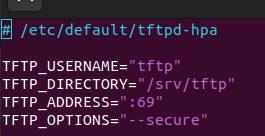
\includegraphics[width=0.5\textwidth]{image/image-20231029162404057.png}
  \caption{tftpd-hpa配置文件修改}
\end{figure}


明确tftp服务器的文件路径在"/srv/tftp", 将上一节生成的work目录下的所有文件拷贝到/srv/tftp路径中。

\section{Uboot 加载 MyKernel 内核和根文件系统}
Uboot 加载MyKernel 内核和根文件系统有两种方法加载。一种是以网络的形式,利用 tftp 协议和 uboot 命令直接将MyKernel 内核和根文件系统加载到内存中,然后手动引导启动。另一种是通过烧录镜像到TF卡的方式。

首先讲解第一种方式:

按照《使用Minicom连接VisionFive2》节中的步骤,连接 VisionFive2 和 Ubuntu 主机,待开发板成功引导 Uboot 后,使用下面的步骤进行配置。

\subsection{配置TFTP服务}

使用网线连接 VisionFive2 开发板后,通过路由器网管查看 Ubuntu 和 VisionFive2 开发板的 IP 地址。并使用以下的命令设置 TFTP 服务器的

\begin{lstlisting}
  setenv serverip 192.168.1.101;
  setenv ipaddr 192.168.1.28;
  setenv getewayip 192.168.1.1;
\end{lstlisting}

在 Uboot中下载 image.fit 文件, 下载速度取决于局域网的带宽,请耐心等待:

\begin{lstlisting}
  tftpboot ${loadaddr} image.fit;
\end{lstlisting}

使用以下命令手动引导内核和根文件系统:
\begin{lstlisting}
  bootm start ${loadaddr};	
  bootm loados ${loadaddr};
  run chipa_set_linux;
  run cpu_vol_set;
  booti ${kernel_addr_r} ${ramdisk_addr_r}:${filesize} ${fdt_addr_r};
\end{lstlisting}

第二种方式相较于第一种方式,几乎不需要在开发板上有任何命令输入。

首先需要准备一张 TF 卡和读卡器,在 VisionFive2 目录中的使用以下命令生成SD 卡 Image 文件:
\begin{lstlisting}
  sudo make -j$(nproc)
  sudo make buildroot_rootfs -j$(nproc)
  sudo make img
\end{lstlisting}

运行完成之后,将在 work目录下产生 sdcard.img 文件。

使用 BalenaEtcher将work 目录中的生成的 sdcard.img 文件烧录至 TF 卡中后, 即可在开发板实现 MyKernel 内核和根文件系统的加载。

MyKernel内核加载后将在开发板上实现一个简单的时间片轮转多道程序,如图下所示:
\begin{figure}[htbp]
  \centering
  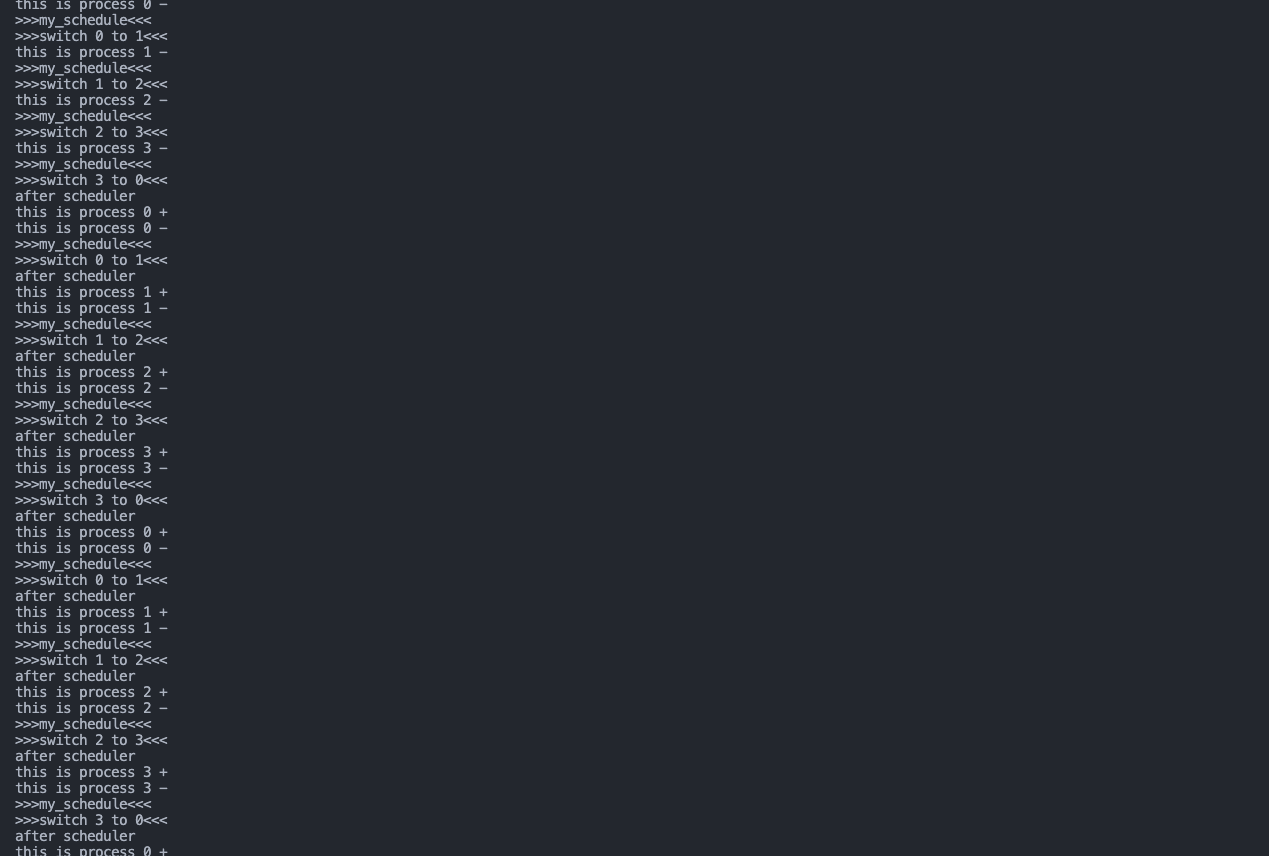
\includegraphics[width=0.7\textwidth]{image/mmexport1701419651344.png}
  \caption{一个简单的时间片轮转多道程序}
\end{figure}


\chapter{实验三:跟踪分析 Linux 内核的启动过程}
\section{下载RISC-V工具链}
对于新手而言,自己克隆RISC-V的仓库进行编译有三大不方便之处:

\begin{enumerate}
  \item RISC-V工具链仓库巨大,对于国内用户下载不方便
  \item RISC-V工具链的依赖包和配置,新手不一定能解决
  \item RISC-V工具链编译时间长
\end{enumerate}

故此,使用他人编译好的工具链,是一种有效的方式。网站 toolchains.bootlin.com 提供了已经编译好的RISC-V工具链,如下图所示:

\begin{figure}[htbp]
  \centering
  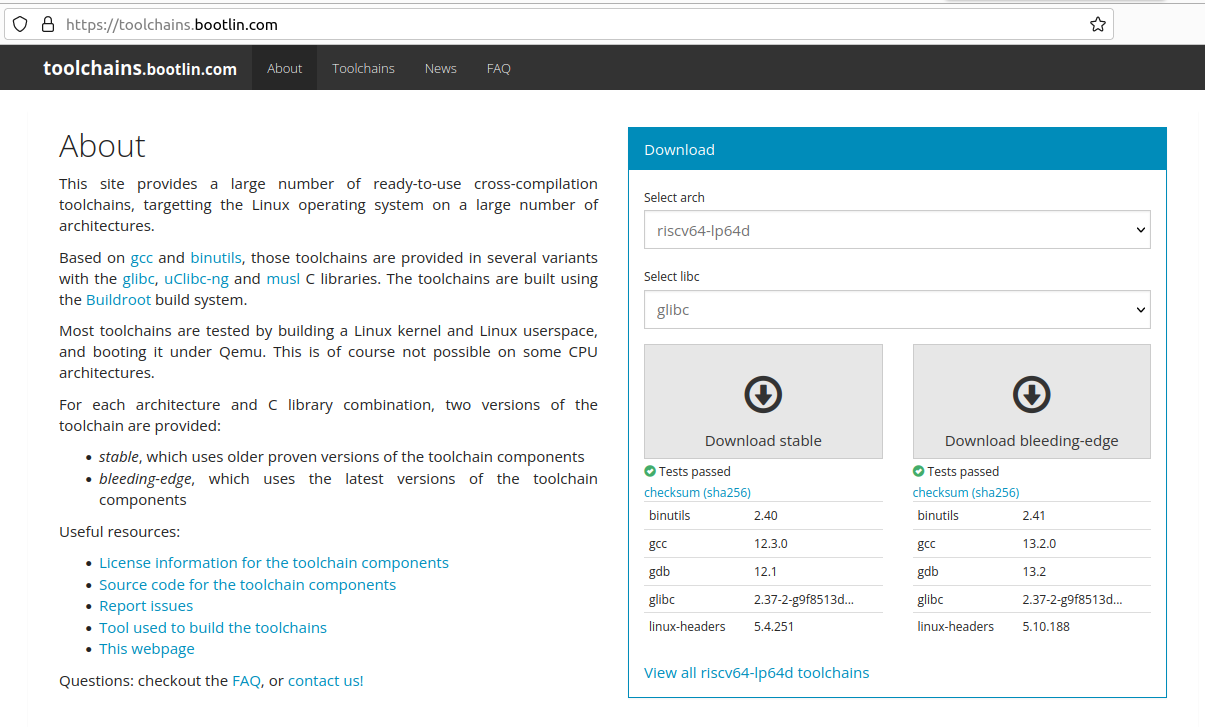
\includegraphics[width=0.7\textwidth]{image/image-20231105091522260.png}
  \caption{RISC-V工具链}
\end{figure}

选项:
\begin{enumerate}

\item 在Select arch选项中,我们选择riscv64-lp64d
\item 在Select libc中选择glibc
\item 下载stable版或者Bleeding-edge
  
\end{enumerate}

本节以下载Bleeding-edge为例。首先使用以下的命令在~目录下创建一个名为的目录:

\begin{lstlisting}
  mkdir riscv64_oslab
  cd riscv64_oslab
\end{lstlisting}

下载之后使用以下的命令进行解压:

\begin{lstlisting}
  wget https://toolchains.bootlin.com/downloads/releases/toolchains/riscv64-lp64d/tarballs/riscv64-lp64d--glibc--bleeding-edge-2023.08-1.tar.bz2
  tar -jxvf riscv64-lp64d--glibc--bleeding-edge-2023.08-1.tar.bz2  
\end{lstlisting}

解压之后,使用你喜欢的编辑器打开位于~目录下的.bashrc或者.zshrc设置工具链的环境变量,下面将使用emacs在zsh下设置工具链的环境变量:

\begin{lstlisting}
  emacs ~/.zshrc
\end{lstlisting}

在.zshrc中添加以下语句:

\begin{lstlisting}
  export PATH=/home/elon/riscv64_oslab/riscv64-lp64d--glibc--bleeding-edge-2023.08-1/bin:$PATH
\end{lstlisting}

需要注意的是 \lstinline{/home/elon} 需要更换为自己的用户名,在\lstinline{riscv64_oslab/riscv64-lp64d--glibc--bleeding-edge-2023.08-1/bin}目录中可使用\lstinline{pwd}命令显示自己需要添加的路径。

\section{安装QEMU}
qemu是一个开源且免费的硬件虚拟化仿真器,可以提供不同的虚拟的计算机架构。我们使用qemu在x86平台上模拟rsicv架构的裸机用于调试和测试linux内核。

在\lstinline{riscv64_oslab}目录下使用以下的命令可以下载和解压qemu:

\begin{lstlisting}
  wget https://download.qemu.org/qemu-7.1.0.tar.xz
  tar xvJf qemu-7.1.0.tar.xz  
\end{lstlisting}

解压后使用以下命令进行配置和编译以及安装:

\begin{lstlisting}
  cd qemu-7.1.0
  ./configure
  make -j$(nproc)	
  make install
\end{lstlisting}

其中\lstinline{make -j$(nproc)}中的\lstinline{-j$(nproc)}参数为以机器硬件线程数进行多线程编译。

\section{编译OpenSBI}
SBI是RISC-V架构下的特权层二进制接口,是用于引导程序环境的规范。通俗的讲就是x86下的bios,但这并不准确,如果想要详细了解什么是OpenSBI,可以参考这个链接OpenSBI Deep Dive。OpenSBI的英文全称是RISC-V Open Source Supervisor Binary Interface 。我们使用OpenSBI引导linux内核的加载。

使用以下的命令在\lstinline{riscv64_oslab}目录下克隆OpenSBI:

\begin{lstlisting}
git clone https://github.com/riscv-software-src/opensbi.git
\end{lstlisting}

使用以下命令进行编译:

\begin{lstlisting}
export CROSS_COMPILE=riscv64-linux-
make PLATFORM=generic -j$(nproc)
\end{lstlisting}
	
最后生成的OpenSBI固件在 \lstinline{build/platform/generic/firmware/} 目录下产生:

\begin{figure}[htbp]
  \centering
  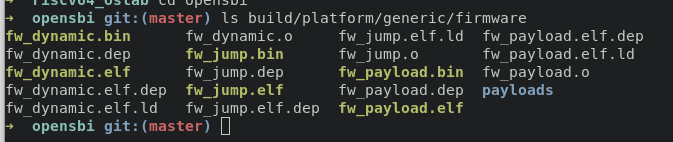
\includegraphics[width=0.7\textwidth]{image/image-20231105093844708.png}
  \caption{产生的OpenSBI固件}
\end{figure}


生成的目录下有三个关键词需要解释:

\begin{enumerate}
\item dynamic:带有动态信息的固件
\item jump:指定下一级的boot地址跳转
\item payload:包含下一级boot的二进制内容,通常是uboot/linux
\end{enumerate}

为了减少工作量,我们不编译uboot,所以我们选择jump关键字的固件 -- \lstinline{fw_jump.elf}.

下图演示了,我们启动Linux内核的次序,与常规方式不同的在于我们使OpenSBI直接jumps跳到Linux Kernel的启动处。

\begin{figure}[htbp]
  \centering
  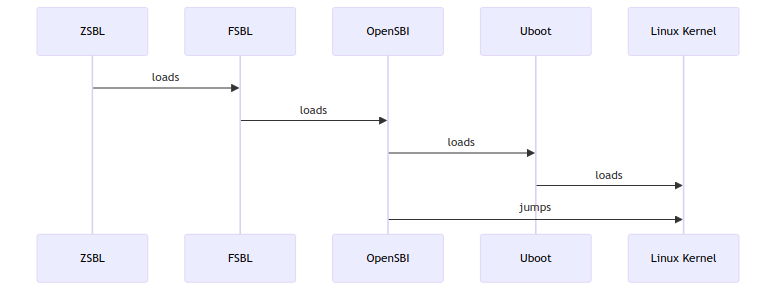
\includegraphics[width=0.7\textwidth]{image/uboot.png}
  \caption{OpenSBI引导操作系统}
\end{figure}


\section{编译Linux Kernel}
由于Linux Kernel在6.0的版本后使用了rust语言进行了编写,为了减少不必要的麻烦和意外,我们使用的Linux内核版本小于v6.0。

使用以下命令在\lstinline{riscv64_oslab}目录下下载和解压Kernel:

\begin{lstlisting}
  wget http://mirrors.besti.net/kernel/v5.x/linux-5.19.16.tar.xz
  tar -xf linux-5.19.16.tar.xz
  cd linux-5.19.16  
\end{lstlisting}

需要注意的是我们使用了电科院的内部Linux Kernel的镜像网站进行下载,读者需要自己的寻找国内的镜像。

解压之后,需要指定编译Linux Kernel的架构和方式。为了编译出RISC-V架构的Linux内核,我们需要指定编译为RISC-V的架构,同时由于我们是在X86的平台上进行编译,所以我们必须使用交叉编译的方式进行编译。命令如下:

\begin{lstlisting}
  export ARCH=riscv
  export CROSS_COMPILE=riscv64-linux-
  make defconfig  
\end{lstlisting}

使用make defconfig后Linux内核目录下会产生一个.config文件,为了方便后面的使用GDB调试RISC-V版本的Linux内核,我们需要为我们编译的内核附加上调试信息。我们需要修改Linux内核目录下的Makefile文件,这里依旧使用emacs进行修改,读者请使用自己喜好的编辑器修改。

\begin{lstlisting}
  emacs Makefile
\end{lstlisting}

在emacs中使用Ctrl+s 粘贴\lstinline{KBUILD_CFLAGS}按下回车,找到\lstinline{KBUILD_CFLAGS}的位置,在后面的选项中加入-g。例如图下:

\begin{figure}[htbp]
  \centering
  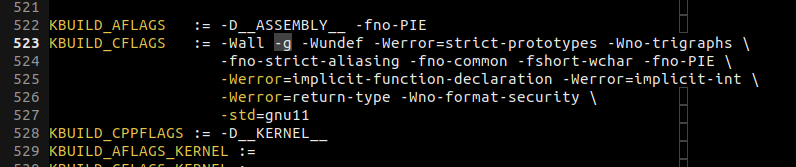
\includegraphics[width=0.7\textwidth]{image/image-20231105100304040.png}
  \caption{修改Makefile}
\end{figure}


此举是为了提供GDB调试的功能。修改完成后保存即可退出,进行最后的编译:

\begin{lstlisting}
  make -j$(nproc)	
\end{lstlisting}

\newpage
编译完成后将在两个地方生成文件。一处就在在linux内核目录下,另一处在linux内核目录下的\lstinline{arch/riscv/boot/},如图所示:

第一处:
\begin{figure}[htbp]
  \centering
  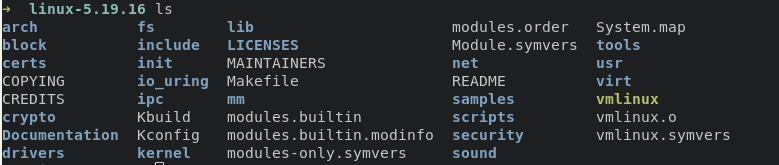
\includegraphics[width=0.7\textwidth]{image/image-20231105100626287.png}
  \caption{linux内核目录}
\end{figure}

第二处:
\begin{figure}[htbp]
  \centering
  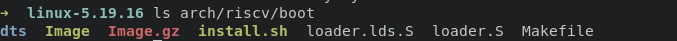
\includegraphics[width=0.7\textwidth]{image/image-20231105100648963.png}
  \caption{boot内核目录}
\end{figure}

\section{制作根文件系统}
一般一个简易的Linux操作系统包括两个部分,一个是Linux Kernel,另一个是根文件系统。制作根文件系统通常有两个工具可以使用,一种是BusyBox,另一种是Buildroot。使用BusyBox制作根文件系统的步骤较多,但是很灵活。而Buildroot操作简单。

首先在\lstinline{riscv64_oslab}目录下下载和解压buildroot:

\begin{lstlisting}
  wget https://buildroot.org/downloads/buildroot-2023.02.6.tar.gz
  tar -xvf buildroot-2023.02.6.tar.gz
\end{lstlisting}

解压后进入buildroot目录进行buildroot配置:

\begin{lstlisting}
  cd buildroot-2023.02.6
  make menuconfig
\end{lstlisting}

\begin{figure}[htbp]
  \centering
  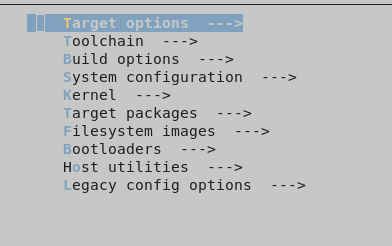
\includegraphics[width=0.3\textwidth]{image/image-20231105101258501.png}
  \caption{Target options}
\end{figure}
使用上述命令将出现一个菜单界面。首先,进入Target options。

\newpage

选择Target Architecture为RISCV。
\begin{figure}[htbp]
  \centering
  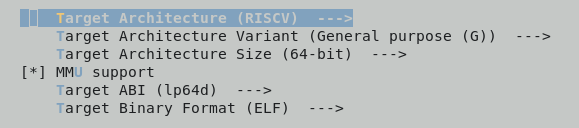
\includegraphics[width=0.4\textwidth]{image/image-20231105101313146.png}
  \caption{选择 RISCV}
\end{figure}

Exit返回一级界面后,选择Filesysem images后选择ext2/3/4 root filesystem。
\begin{figure}[htbp]
  \centering
  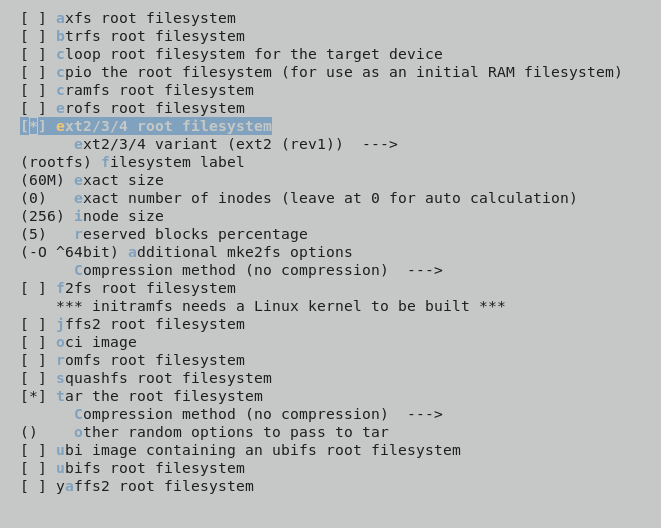
\includegraphics[width=0.4\textwidth]{image/image-20231105101339834.png}
  \caption{选择  root filesystem}
\end{figure}

保存后使用以下命令进行编译:

\begin{lstlisting}
  make -j\$(nproc)	
\end{lstlisting}

本次编译由于buildroot需要编译自己的编译需要的工具链,因此时间较长,请读者耐心等待。编译完成后,在output/images目录下将生成我们需要的文件。

\begin{figure}[htbp]
  \centering
  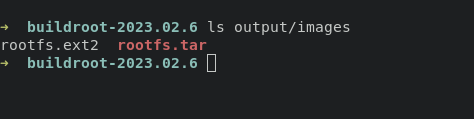
\includegraphics[width=0.7\textwidth]{image/image-20231105101948270.png}
  \caption{output files}
\end{figure}

至此,漫长的编译过程已经结束了。下一节,我们将运行自己制作的一个简易linux操作系统和进行GDB远程调试内核,从start\_kernel到init进程启动。

\section{运行简易Linux内核}
使用以下命令在\lstinline{riscv64_oslab}目录创建images目录:

\begin{lstlisting}
  mkdir images
\end{lstlisting}

使用以下命令在images目录下将之前各个部分的编译好的文件复制到images目录下:

\begin{lstlisting}
  cp ../opensbi/build/platform/generic/firmware/fw_jump.elf .
  cp ../linux-5.19.16/vmlinux .
  cp ../linux-5.19.16/arch/riscv/boot/Image .
  cp ../buildroot-2023.02.6/output/images/rootfs.ext2 .
\end{lstlisting}

复制完后images目录下将产生以下文件:


\begin{figure}[htbp]
  \centering
  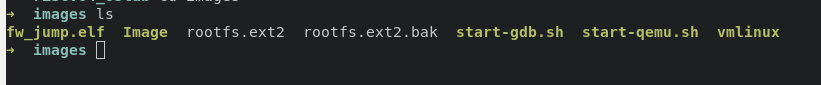
\includegraphics[width=0.7\textwidth]{image/image-20231105102806931.png}
  \caption{images output files}
\end{figure}

现在需要编译一个名叫start-qemu.sh的shell脚本。

使用你喜欢的编辑器打开start-qemu.sh,填写下以下内容。这里仍然使用emacs作为示例:

\begin{lstlisting}
  emacs start-qemu.sh
\end{lstlisting}

内容如下:


\begin{lstlisting}
  #!/bin/sh

  qemu-system-riscv64 -M virt \
  -bios fw_jump.elf \
  -kernel Image \
  -append "rootwait root=/dev/vda ro" \
  -drive file=rootfs.ext2,format=raw,id=hd0 \
  -device virtio-blk-device,drive=hd0 \
  -netdev user,id=net0 -device virtio-net-device,netdev=net0 -nographic
\end{lstlisting}

使用以下命令给start-qemu.sh赋予执行权:

\begin{lstlisting}
  chmod +x start-qemu.sh
\end{lstlisting}

使用以下命令即可运行简易的RISC-V架构的简易Linux操作系统:

\begin{lstlisting}
  ./start-qemu.sh
\end{lstlisting}

\newpage
启动界面如下:
\begin{figure}[htbp]
  \centering
  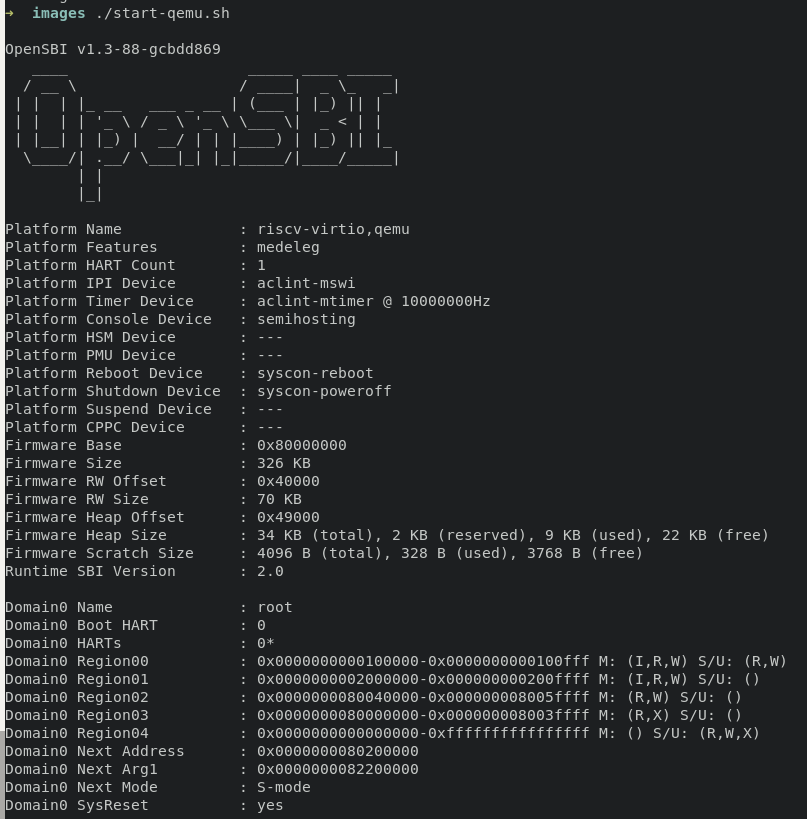
\includegraphics[width=0.3\textwidth]{image/image-20231105103328525.png}
  \caption{启动界面}
\end{figure}

加载完后显示用户登录:
\begin{figure}[htbp]
  \centering
  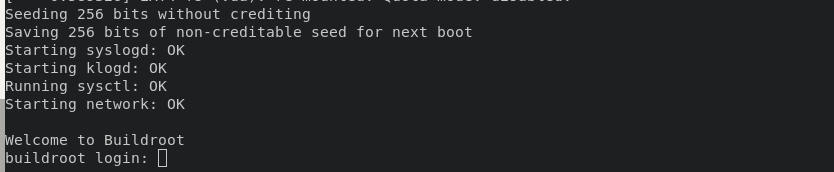
\includegraphics[width=0.7\textwidth]{image/image-20231105103401143.png}
  \caption{用户登录}
\end{figure}

输入root点击回车,进入shell。
\begin{figure}[htbp]
  \centering
  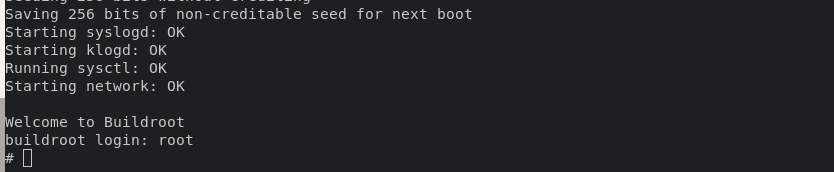
\includegraphics[width=0.7\textwidth]{image/image-20231105103508731.png}
  \caption{进入shell}
\end{figure}

从start\_kernel到init进程启动
上节,我们已经完成了在qemu上运行一个简易的RISC-V架构的Linux操作系统。这一节,将对这个Linux内核进行调试。

使用你喜欢的编辑器创建 start-gdb.sh shell脚本,按照惯例,笔者依旧使用emacs。

\begin{lstlisting}
  emacs ./start-gdb.sh
\end{lstlisting}
脚本内容如下:

\begin{lstlisting}
  qemu-system-riscv64 -M virt \
  -bios fw_jump.elf \
  -kernel Image \
  -append "rootwait root=/dev/vda ro" \
  -drive file=rootfs.ext2,format=raw,id=hd0 \
  -device virtio-blk-device,drive=hd0 \
  -netdev user,id=net0 -device virtio-net-device,netdev=net0 \
  -nographic \
  -s -S
\end{lstlisting}
保存后,使用以下的命令对start-gdb.sh赋予执行权:

\begin{lstlisting}
  chmod +x ./start-gdb.sh
\end{lstlisting}

使用以下命令安装 gdb-multiarch 为接下来的调试做准备:
\begin{lstlisting}
  sudo apt install gdb-multiarch
\end{lstlisting}

现在我们开始正式调试RISC-V架构的Linux内核。

首先在images目录下使用以下命令,启动qemu并开启远程调试:
\begin{lstlisting}
  ./start-gdb.sh
\end{lstlisting}

然后打开另一个终端,进入imags目录后使用以下命令进入gdb:

\begin{lstlisting}
  gdb-multiarch ./vmlinux
\end{lstlisting}

进入gdb后显示:\lstinline{Reading symbols from ./vmlinux...} 说明操作正常,可以进一步操作:

\begin{figure}[htbp]
  \centering
  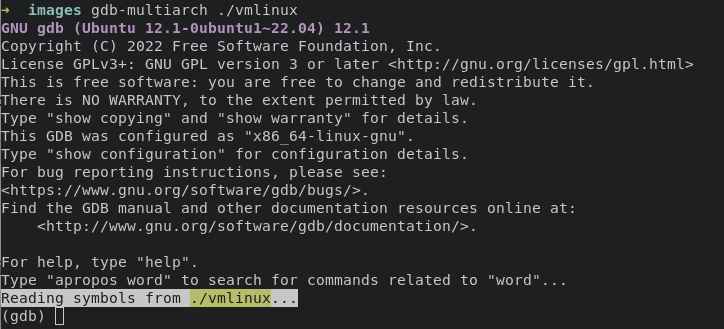
\includegraphics[width=0.7\textwidth]{image/image-20231105111831194.png}
  \caption{进入gdb}
\end{figure}

现在在gdb内输入以下命令后回车:

\begin{lstlisting}
  target remote:1234
\end{lstlisting}

此举是为了建立gdb和在qemu中启动的gdbserver之间的连接。连接完毕后显示如下:

\begin{figure}[htbp]
  \centering
  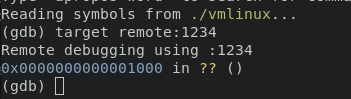
\includegraphics[width=0.7\textwidth]{image/image-20231105112104038.png}
  \caption{建立gdb连接}
\end{figure}

说明建立连接成功。

\newpage
现在使用以下命令gdb对start\_kernel进行打断点:

\begin{lstlisting}
  break start_kernel
\end{lstlisting}

gdb显示start\_kernel函数在\lstinline{init/main.c}文件中。

\begin{figure}[htbp]
  \centering
  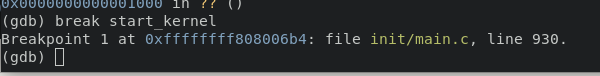
\includegraphics[width=0.7\textwidth]{image/image-20231105112248991.png}
  \caption{gdb显示start\_kernel函数}
\end{figure}


使用c命令让程序执行到start\_kernel断点处:
\begin{figure}[htbp]
  \centering
  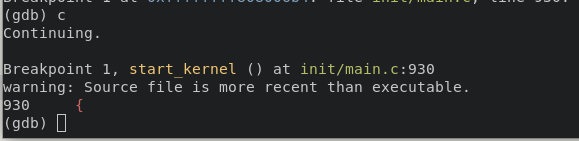
\includegraphics[width=0.7\textwidth]{image/image-20231105112437905.png}
  \caption{执行到start\_kernel断点处}
\end{figure}

现在使用l命令显示start\_kernel断点处:
\begin{figure}[htbp]
  \centering
  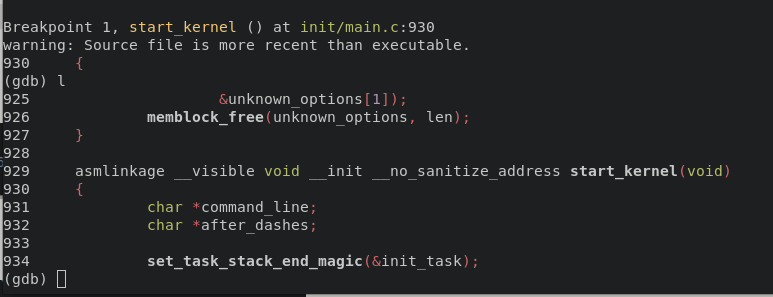
\includegraphics[width=0.7\textwidth]{image/image-20231105112512318.png}
  \caption{显示start\_kernel断点处信息}
\end{figure}

l命令显示start\_kernel函数位于\lstinline{init/main.c}中的930行。

在Linux 内核的进程树中,涉及到三个重要的进程,分别是 0号进程 和 1号进程 以及 2号进程 。示意图如下所示:

\begin{figure}[htbp]
  \centering
  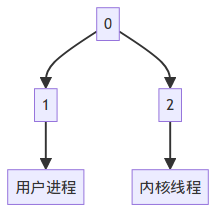
\includegraphics[width=0.3\textwidth]{image/jc.png}
  \caption{进程示意图}
\end{figure}

\newpage
0号进程 是通过手动创建的,在\lstinline{start_kernel} 中出现的 \lstinline{&init_task} 就是 0号进程 的进程描述符。

接下来,让我们先使用编辑器打开linux-5.19.16中init目录中的main.c文件找到\lstinline{asmlinkage __visible void __init __no_sanitize_address start_kernel(void)}。让我们一起阅读\lstinline{start_kernel}函数的Linux内核源码。

在这部分的源码中的1138行,也就是start\_kernel函数的倒数第二个函数,有一个名叫 \lstinline{arch_call_rest_init()}的函数。 \lstinline{arch_call_rest_init()} 的定义如下:

\begin{lstlisting}
  void __init __weak arch_call_rest_init(void)
  {
    rest_init();
  }
\end{lstlisting}

我们在gdb中不断使用n命令,当next到了 \lstinline{arch_call_rest_init} 时, 内核即将创建\lstinline{kernel_init 1}号进程和 kthreadd 2号进程。
\begin{figure}[htbp]
  \centering
  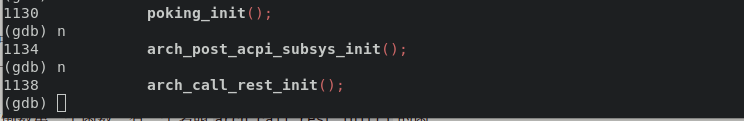
\includegraphics[width=0.7\textwidth]{image/image-20231105113449231.png}
  \caption{arch\_call\_rest\_init}
\end{figure}

\newpage
使用\lstinline{b rest_init} 对\lstinline{rest_init()}函数进行打断点,进入 rest\_init 函数后如下:
\begin{figure}[htbp]
  \centering
  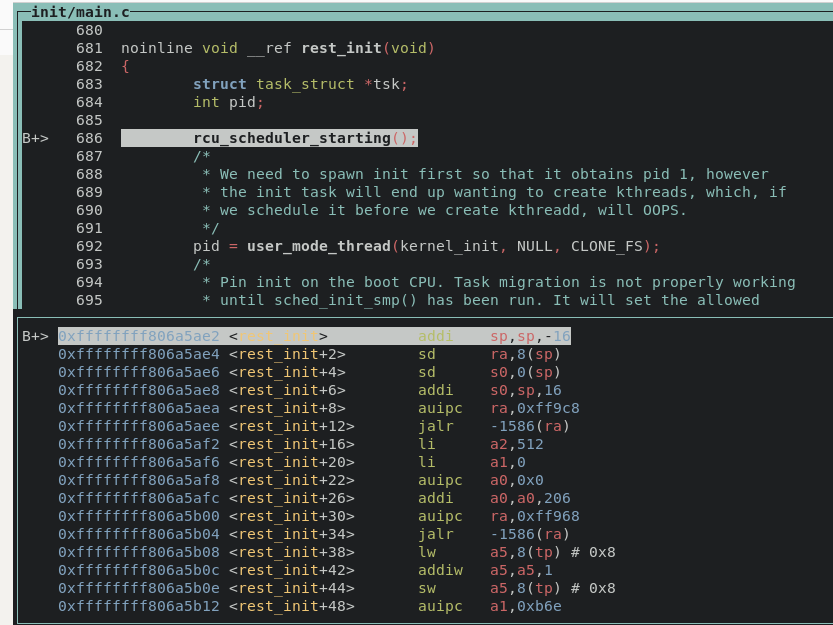
\includegraphics[width=0.7\textwidth]{image/image-20231111155131309.png}
  \caption{rest\_init}
\end{figure}


此时执行下一步会出现调用 user\_mode\_thread , 此时这个函数就是创建 1号进程,而 1号进程 也被称为 init 进程 。继续向下单步执行, 会发现调用 \lstinline{kernel_thread},这个函数就是用于创建 2号进程 ,即内核线程。

此时再使用c命令,将完成Linux Kernel引导,系统进入登录界面:
\begin{figure}[htbp]
  \centering
  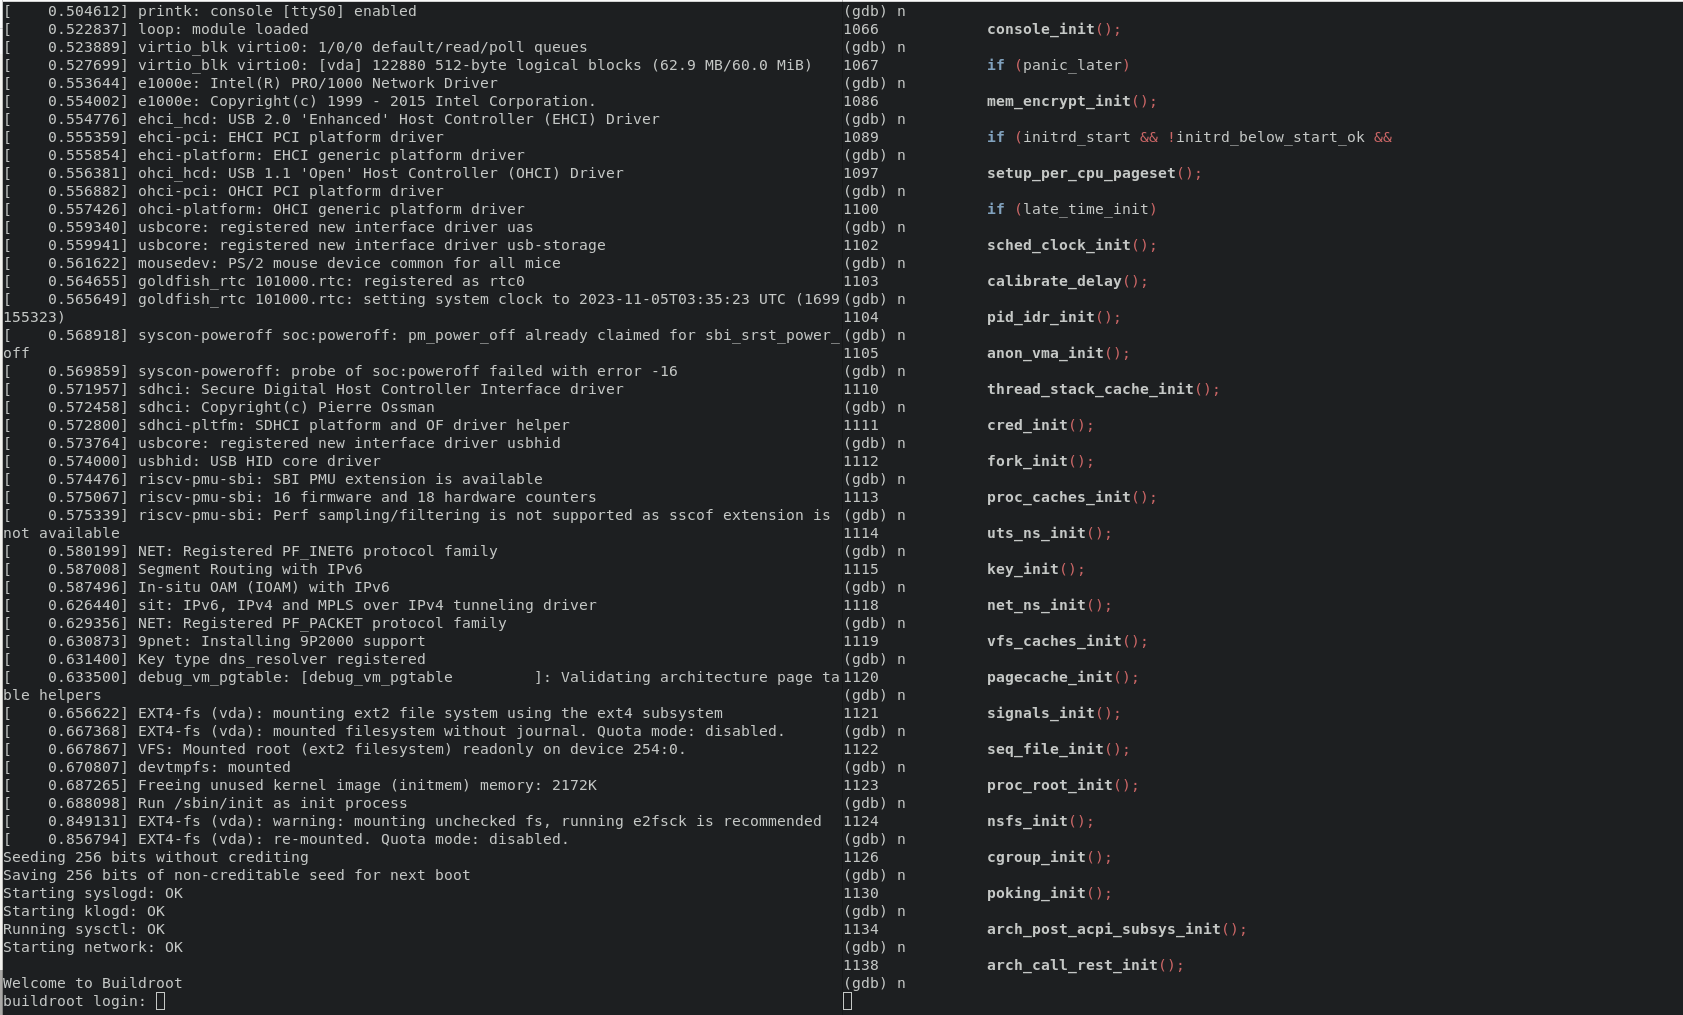
\includegraphics[width=0.7\textwidth]{image/image-20231105113622844.png}
  \caption{进入登录界面}
\end{figure}

至此调试结束。

start-kernel 函数中包括了内核的初始化和一系列的设置,包括文件系统、调度器、定时器、内存管理、锁初始化、内存加密、NUMA 策略、ACPI 初始化等等。而 \lstinline{rest_init} 函数宣告了初始化的结束。

\chapter{实验四:使用库函数API和C代码中嵌入汇编代码两种方式使用同一个系统调用}
\section{使用SSH连接starfive visionfive 2}
在第一个实验中,我们配置好了使用 ssh 连接 starfive visionfive 2 开发板的流程。在连接好网线后,通过使用浏览器登录网管地址查看开发板的ip地址后,使用以下命令连接 starfive visionfive 2 开发板。

\begin{lstlisting}
  ssh root@192.168.xxx.xxx
\end{lstlisting}

注意:\lstinline{192.168.xxx.xxx } Ip地址需要使用自己查阅的Ip地址。

回车后,输入密码: starfive。进入 starfive visionfive 2 开发板中的shell。如下图所示:

\begin{figure}[htbp]
  \centering
  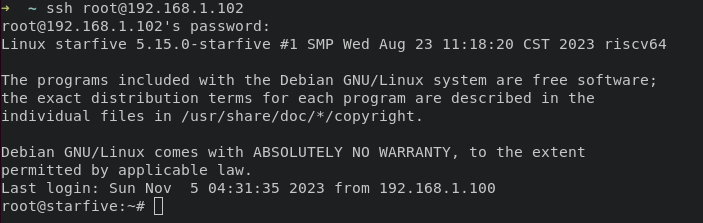
\includegraphics[width=0.7\textwidth]{image/image-20231105133005556.png}
  \caption{ starfive visionfive 2 Shell}
\end{figure}

\section{使用man查看write函数}
使用以下命令查看write函数的具体用法

\lstinline{man 2 write}
具体用法如图所示:
\begin{figure}[htbp]
  \centering
  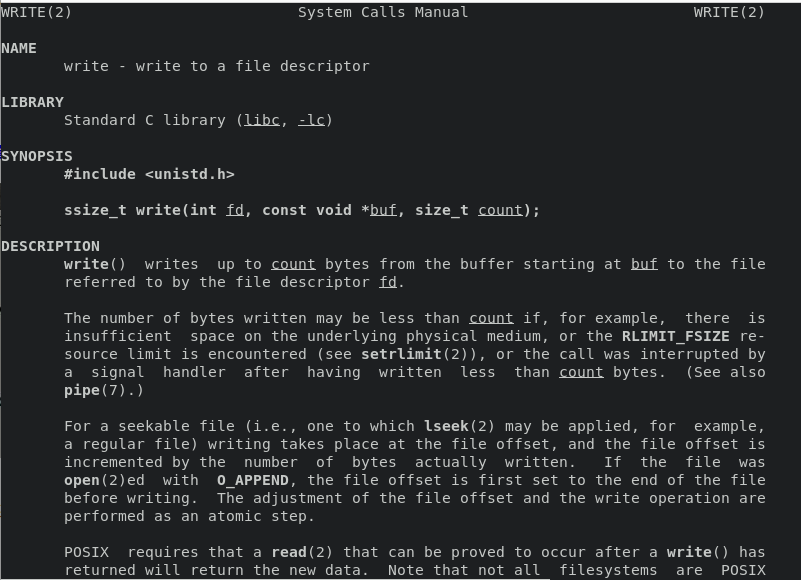
\includegraphics[width=0.7\textwidth]{image/image-20231105133327813.png}
  \caption{man 2 write}
\end{figure}

write函数有三个参数。第0个参数,输出位置;第1个参数,指向输出内容的指针;第2个参数,输出内容的长度。

\section{C语言调用write函数}
接下来,我们将在shell中vim编写local\_write.c程序,通过使用C语言调用write函数。

首先我们需要下载 vim, 使用以下命令下载安装 vim 。

\begin{lstlisting}
  sudo apt install vim
\end{lstlisting}

安装好后,使用以下命令创建 local\_write.c 文件。

\begin{lstlisting}
  vim loacl_write.c
\end{lstlisting}

将下面的代码复制到 local\_write.c 中:

\begin{lstlisting}
  #include <stdio.h>
  #include <unistd.h>
  int main(void){
    char s[]="hello, world.\n";
    write(1,s,13);
    return 0;
  }
\end{lstlisting}

使用以下命令进行编译和运行:

\begin{lstlisting}
gcc -o loacl_write -c local_wirte.c
./local_write
\end{lstlisting}

显示以下信息说明运行成功:
\begin{figure}[htbp]
  \centering
  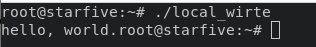
\includegraphics[width=0.5\textwidth]{image/image-20231105134051213.png}
  \caption{local\_wirte运行成功}
\end{figure}

\section{RISC-V内联汇编调用write函数}
接下来,我们将使用RISC-V内联汇编嵌入C语言代码中,调用write函数。

使用以下命令创建 asm\_write.c 文件。

\begin{lstlisting}
  vim asm_write.c
\end{lstlisting}

将下面的代码复制到 asm\_write.c 中:

\begin{lstlisting}
  #include <stdio.h>
  #include <unistd.h>

  int main() {
    char s[] = "hello, world\n";

    __asm__ volatile(
    "li a2, 13\n"
    "li a0, 1\n"
    "mv a1, %[str]\n"
    "li a7, 64\n"	
    "ecall \n"
    :
    : [str] "r" (s)	
    );

    return 0;
  }
\end{lstlisting}

使用以下命令进行编译和运行:

\begin{lstlisting}
  gcc -o asm_write -c asm_write.c
  ./asm_write
\end{lstlisting}

显示以下信息说明运行成功:
\begin{figure}[htbp]
  \centering
  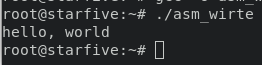
\includegraphics[width=0.5\textwidth]{image/image-20231105134323745.png}
  \caption{asm\_write运行成功}
\end{figure}

\section{内联汇编解释}
可能最开始有很多不了解的人会认为系统调用和函数调用差不多,然而当我们用汇编代码运行了第一个系统调用之后就会发现这个步骤和函数调用还是很不同的,即使他们在你是使用库函数的时候感觉是差不多的。它没有函数的入口,也没有函数的出口(请看lab2中的资料),而且还多了一个ecall。那么系统调用是怎么运行的呢?

抽象系统资源
为了完全明白这段汇编代码,让我们先了解一点前置的知识。

当谈及操作系统时,人们可能会问的第一个问题是为什么需要它?也就是说,我们可以将所有的系统调用实现为一个库,应用程序可以与之链接。在此方案中,每个应用程序甚至可以根据自己的需求定制自己的库。应用程序可以直接与硬件资源交互,并以应用程序的最佳方式使用这些资源(例如,实现高性能或可预测的性能)。一些嵌入式设备或实时系统的操作系统就是这样组织的。

这种库函数方法的缺点是,如果有多个应用程序在运行,这些应用程序必须表现良好。例如,每个应用程序必须定期放弃中央处理器,以便其他应用程序能够运行。如果所有应用程序都相互信任并且没有错误,这种协同操作的分时方案可能是可以的。 然而更典型的情况是, 应用程序互不信任且存在bug,所以人们通常希望提供比合作方案更强的隔离。

为了实现强隔离, 最好禁止应用程序直接访问敏感的硬件资源,而是将资源抽象为服务。 例如,Unix应用程序只通过文件系统的open、read、write和close系统调用与存储交互,而不是直接读写磁盘。这为应用程序提供了方便实用的路径名,并允许操作系统(作为接口的实现者)管理磁盘。即使隔离不是一个问题,有意交互(或者只是希望互不干扰)的程序可能会发现文件系统比直接使用磁盘更方便。

同样,Unix在进程之间透明地切换硬件处理器,根据需要保存和恢复寄存器状态,这样应用程序就不必意识到分时共享的存在。这种透明性允许操作系统共享处理器,即使有些应用程序处于无限循环中。

另一个例子是,Unix进程使用exec来构建它们的内存映像,而不是直接与物理内存交互。这允许操作系统决定将一个进程放在内存中的哪里;如果内存很紧张,操作系统甚至可以将一个进程的一些数据存储在磁盘上。exec还为用户提供了存储可执行程序映像的文件系统的便利。

linux系统调用接口是精心设计的,既为程序员提供了便利,又提供了强隔离的可能性。Unix接口不是抽象资源的唯一方法,但它已经被证明是一个非常好的方法

用户态,内核态,以及系统调用
强隔离需要应用程序和操作系统之间的硬边界,如果应用程序出错,我们不希望操作系统失败或其他应用程序失败,相反,操作系统应该能够清理失败的应用程序,并继续运行其他应用程序,要实现强隔离,操作系统必须保证应用程序不能修改(甚至读取)操作系统的数据结构和指令,以及应用程序不能访问其他进程的内存。

CPU为强隔离提供硬件支持。例如,RISC-V有三种CPU可以执行指令的模式:机器模式(Machine Mode)、用户模式(User Mode)和管理模式(Supervisor Mode)。在机器模式下执行的指令具有完全特权;CPU在机器模式下启动,OpenSBI也是运行在机器模式下的。操作系统运行在管理模式,用户程序运行在用户模式。

在管理模式下,CPU被允许执行特权指令:例如,启用和禁用中断、读取和写入保存页表地址的寄存器等。如果用户模式下的应用程序试图执行特权指令,那么CPU不会执行该指令,而是切换到管理模式,以便管理模式代码可以终止应用程序,因为它做了它不应该做的事情。应用程序只能执行用户模式的指令(例如,数字相加等),并被称为在用户空间中运行,而此时处于管理模式下的软件可以执行特权指令,并被称为在内核空间中运行。在内核空间(或管理模式)中运行的软件被称为内核。

想要调用内核函数的应用程序(例如上面的write系统调用)必须过渡到内核。CPU提供一个特殊的指令,将CPU从用户模式切换到管理模式,并在内核指定的入口点进入内核(RISC-V为此提供ecall指令)。一旦CPU切换到管理模式,内核就可以验证系统调用的参数,决定是否允许应用程序执行请求的操作,然后拒绝它或执行它。由内核控制转换到管理模式的入口点是很重要的;如果应用程序可以决定内核入口点, 那么恶意应用程序可以在跳过参数验证的地方进入内核。

write调用的汇编代码
现在我们已经明白了使用系统调用的原因。那么理解起来这段汇编代码就很简单了。首先我们需要将参数填入合适的位置,write系统调用的第一个参数是写在哪,需要我们传入文件描述符。第二个参数是写入的字符串的指针。第三个参数是写入字符串的长度。我们将每个值按照相应的方法
\begin{lstlisting}
  "li a2, 13\n" 
  "li a0, 1\n" 
  "mv a1, %[str]\n"
\end{lstlisting}

加载进寄存器(这部分是和函数调用是一样的),然后接下来我们需要陷入到内核态,在RISCV里面我们使用的是ecall。我们将ecall写上,但是此时系统并不知道我们是什么系统调用,所以我们需要在a7寄存器里面加入我们的系统调用号64。自此系统调用的代码我们就完成了。

\chapter{实验五:分析 system call 中断处理过程}

\section{MenuOS迁移到RISC-V架构}
MenuOS 是接下来四次实验的平台。但是由于MenuOS原本设计是为x86架构所服务的,如果需要在RISC-V架构上的机器上运行,就必须对关键部分的汇编代码进行修改。

首先使用以下命令克隆MenuOS:

\begin{lstlisting}
  cd ~/riscv64_oslab/
  mkdir MenuOS
  cd MenuOS
  git clone https://github.com/mengning/menu.git
\end{lstlisting}

克隆后,进入menu目录,使用你喜欢的编辑器对其中的TimeAsm函数进行修改,修改内容如下:

\begin{lstlisting}
  int TimeAsm(int argc, char *argv[])
  {
    time_t tt;
    struct tm *t;
    asm volatile(
    "li a0,201\n\t"
    "ecall \n\t"
    "sd a0, %0\n\t"
    : "=m" (tt)
    );
    t = localtime(&tt);
    printf("time:%d:%d:%d:%d:%d:%d\n",t->tm_year+1900, t->tm_mon, t->tm_mday, t->tm_hour, t->tm_min, t->tm_sec);
    return 0;
  }
\end{lstlisting}
另外一个需要修改的文件是Makefile,这个文件的修改非常重要,将决定产生的什么架构的执行文件。

同样,请使用你喜欢的编辑器,打开Makefile,将其修改为以下内容:

\begin{lstlisting}
  #
  # Makefile for Menu Program
  #

  CC_PTHREAD_FLAGS			 = -lpthread
  CC_FLAGS                     = -c 
  CC_OUTPUT_FLAGS				 = -o
  CC                           = riscv64-linux-gcc
  RM                           = rm
  RM_FLAGS                     = -f

  TARGET  =   test
  OBJS    =   linktable.o  menu.o test.o

  all:	$(OBJS)
  $(CC) $(CC_OUTPUT_FLAGS) $(TARGET) $(OBJS) 
  rootfs:
  riscv64-linux-gcc -o init linktable.c menu.c test.c  -static -lpthread
  riscv64-linux-gcc -o hello hello.c -static
  find init hello | cpio -o -Hnewc |gzip -9 > ../rootfs.img
  qemu-system-riscv64 -M virt \
  -kernel ../linux-5.19.16/arch/riscv/boot/Image \
  -initrd ../rootfs.img \
  -nographic
  .c.o:
  $(CC) $(CC_FLAGS) $<

  clean:
  $(RM) $(RM_FLAGS)  $(OBJS) $(TARGET) *.bak
\end{lstlisting}
需要注意的是,本次实验需要使用 qemu-system-riscv64 和 qemu-system-riscv64 , 请完成第三次实验后,再来做此次实验。

使用以下命令进行编译和运行:

\begin{lstlisting}
  make -j$(nproc)
  make rootfs -j$(nproc)
\end{lstlisting}
成功运行后,将会显示以下信息:
\begin{figure}[htbp]
  \centering
  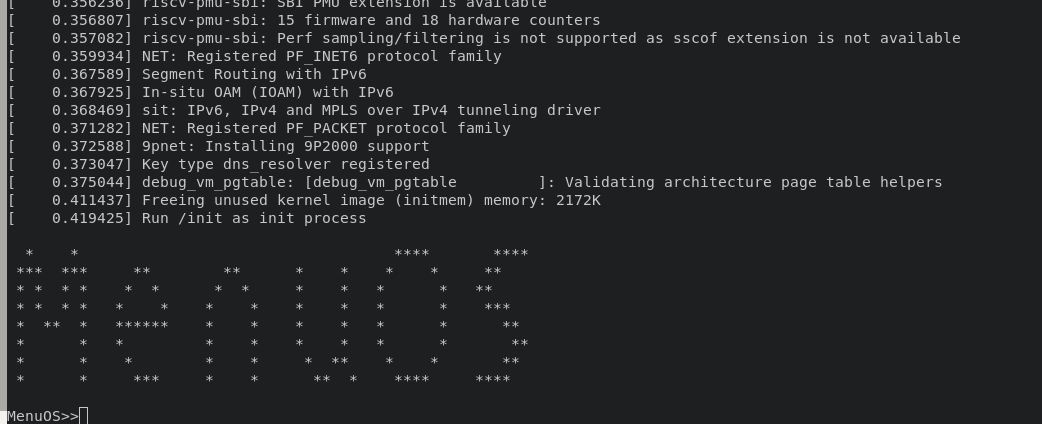
\includegraphics[width=0.7\textwidth]{image/image-20231105212015685.png}
  \caption{编译和运行}
\end{figure}


\section{CWrite和的编写}
现在我们在menu目录下, 使用你喜欢的编辑器修改test.c。这里使用神之编辑器emacs进行修改。

\begin{lstlisting}
  emacs test.c
\end{lstlisting}
打开之后,添加以下内容:

CWrite函数内容如下:

\begin{lstlisting}
  int CWrite(void){
    char s[]="hello, world\n";
    write(1,s,13);
    return 0;
    return 0;
  }
\end{lstlisting}

WriteAsm函数如下:


\begin{lstlisting}
  int WriteAsm(void){
    char s[] = "hello, world\n";

    __asm__ volatile(
    "li a2, 13\n"
    "li a0, 1\n"
    "mv a1, %[str]\n"
    "li a7, 64\n"
    "ecall \n"
    :
    : [str] "r" (s)
    );
    return 0;
  }
\end{lstlisting}

同样使用以下命令进行编译和运行:

\begin{lstlisting}
  make -j$(nproc)
  make rootfs -j$(nproc)
\end{lstlisting}

启动MenuOS后:

输入 help 后回车,显示如下信息:
\begin{figure}[htbp]
  \centering
  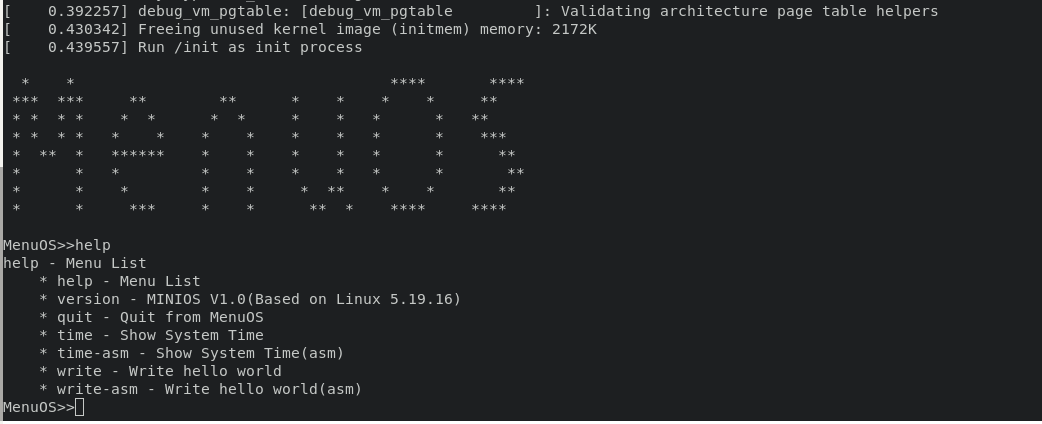
\includegraphics[width=0.7\textwidth]{image/image-20231105212850985.png}
  \caption{MenuOS help}
\end{figure}

再次输入 write 后回车,MenuOS输出以下信息:
\begin{figure}[htbp]
  \centering
  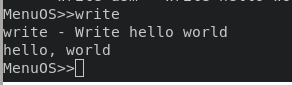
\includegraphics[width=0.7\textwidth]{image/image-20231105212959159.png}
  \caption{MenuOS write}
\end{figure}

输入 write-asm 后回车,MenuOS输出以下信息:
\begin{figure}[htbp]
  \centering
  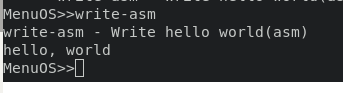
\includegraphics[width=0.7\textwidth]{image/image-20231105213246034.png}
  \caption{MenuOS write-asm}
\end{figure}

\section{GDB调试sys\_write函数}
使用你喜欢的编辑器在menu目录下,编写start-gdb.sh ,这里依旧使用emacs。

start-gdb.sh 的内容如下:

\begin{lstlisting}
  #!/bin/sh
  qemu-system-riscv64 -M virt \
  -kernel ../linux-5.19.16/arch/riscv/boot/Image \
  -initrd ../rootfs.img \
  -nographic \
  -s -S
\end{lstlisting}

使用以下命令赋予start-gdb.sh 执行的权限:

\begin{lstlisting}
  chmod +x start-gdb.sh
\end{lstlisting}
使用以下命令启动 start-gdb.sh:

\begin{lstlisting}
  ./start-gdb.sh
\end{lstlisting}
启动后,shell中应当不显示任何内容,如下所示:
\begin{figure}[htbp]
  \centering
  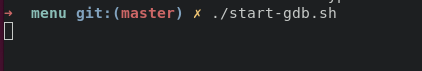
\includegraphics[width=0.7\textwidth]{image/image-20231105221503598.png}
  \caption{start-gdb.sh}
\end{figure}

另开一个终端,进入MenuOS的目录下,使用以下命令启动 gdb-multiarch  。
\begin{lstlisting}
  gdb-multiarch linux-5.19.16/vmlinux
\end{lstlisting}
启动之后,输入 target remote:1234 建立连接,显示如下信息说明连接建立完成:
\begin{figure}[htbp]
  \centering
  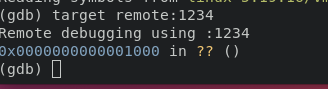
\includegraphics[width=0.7\textwidth]{image/image-20231105221724247.png}
  \caption{target remote:1234}
\end{figure}

依次使用以下命令进行 sys\_write 的调试:
\begin{lstlisting}
  b sys_write
  c
  layout split
\end{lstlisting}
最终界面将显示如下信息:
\begin{figure}[htbp]
  \centering
  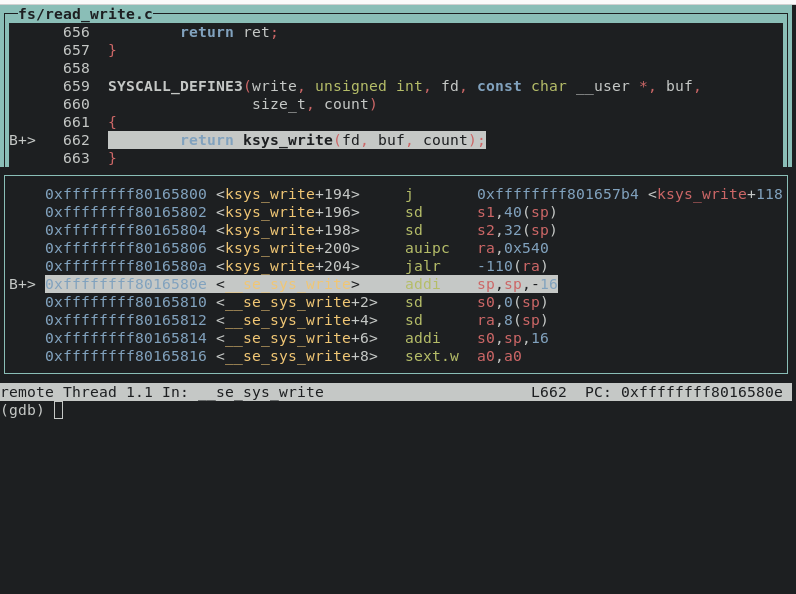
\includegraphics[width=0.7\textwidth]{image/image-20231105221933745.png}
  \caption{最终界面}
\end{figure}


此时,将启动 gdb-multiarch 的终端和启动 ./start-gdb.sh 的终端分别分屏左右,方便查看调试过程中的程序的输出,如下图所示:
\begin{figure}[htbp]
  \centering
  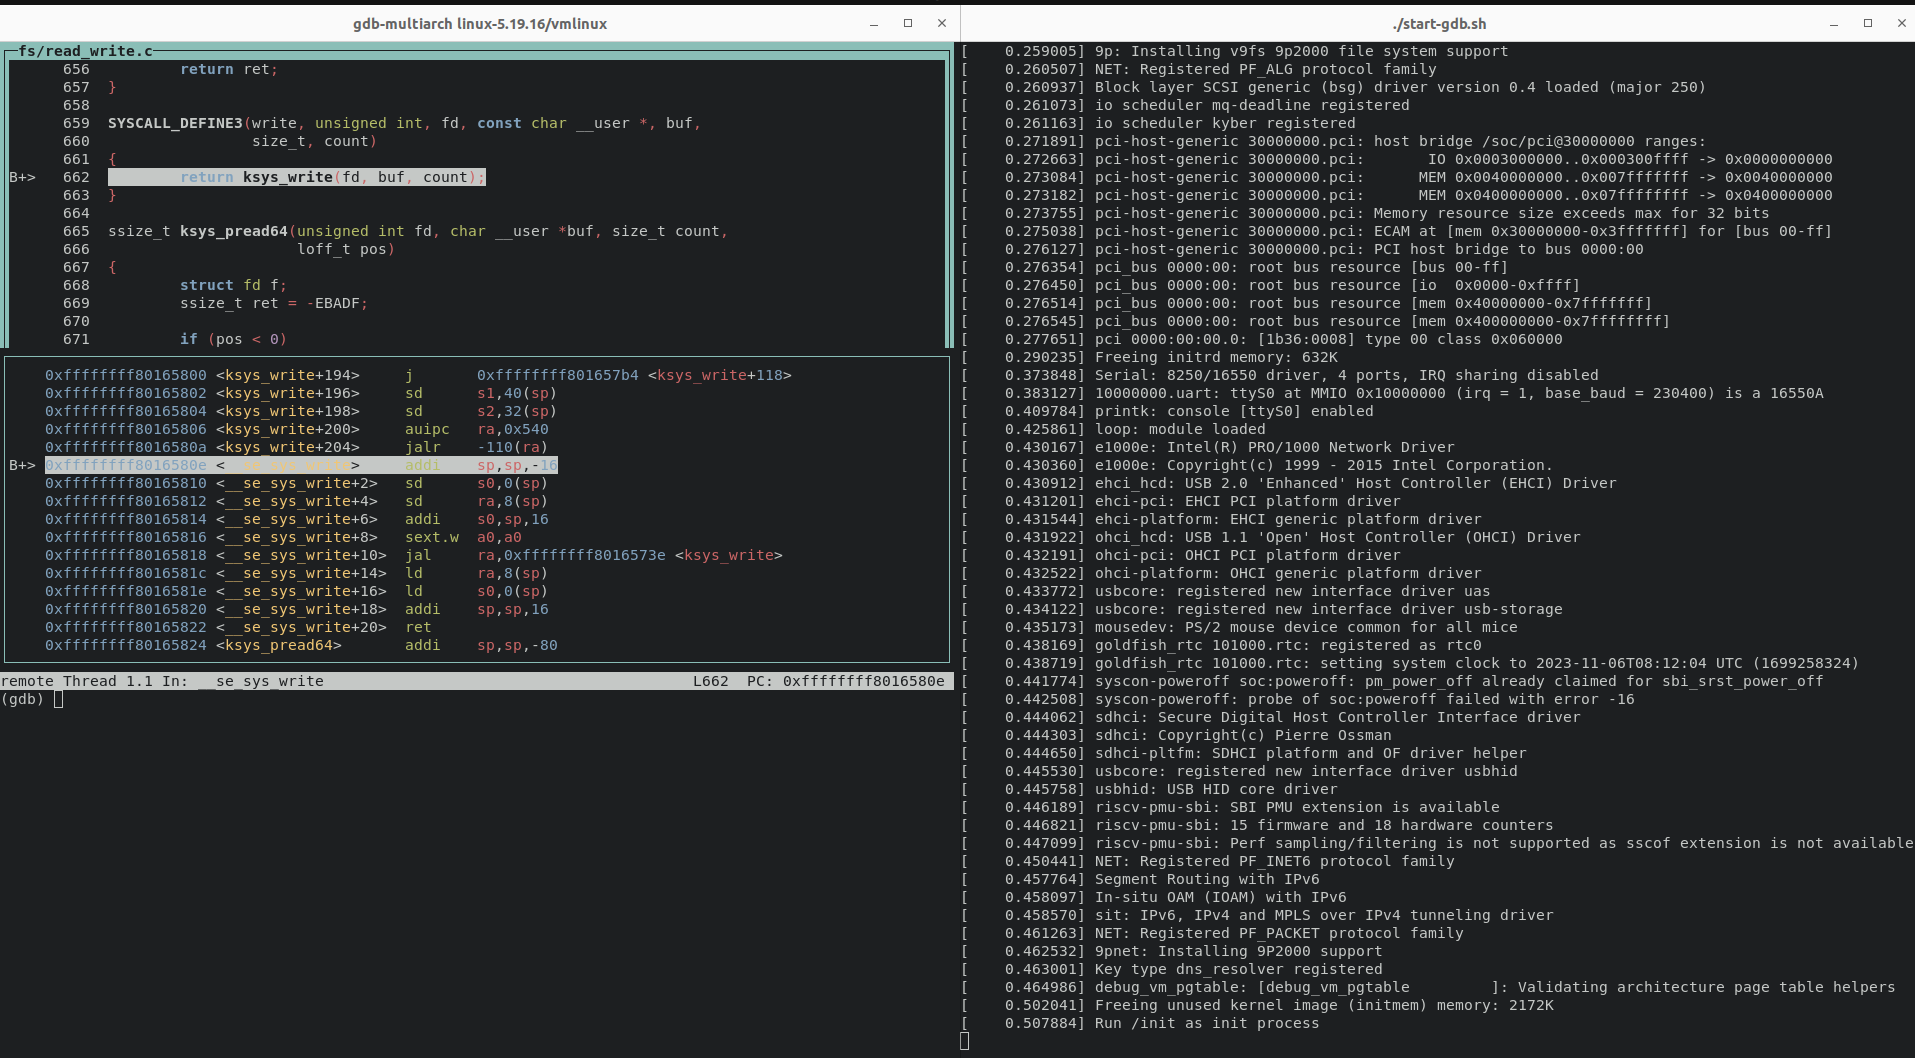
\includegraphics[width=0.7\textwidth]{image/image-20231106161606896.png}
  \caption{gdb分屏}
\end{figure}

\newpage
执行上面打断点的操作后,在右侧图中的的最后一行显示:[    0.507884] Run /init as init process 说明Linux 内核已经初始化完成。 现在使用 十一次 c 命令,使得MenuOS加载到shell,如下图所示:
\begin{figure}[htbp]
  \centering
  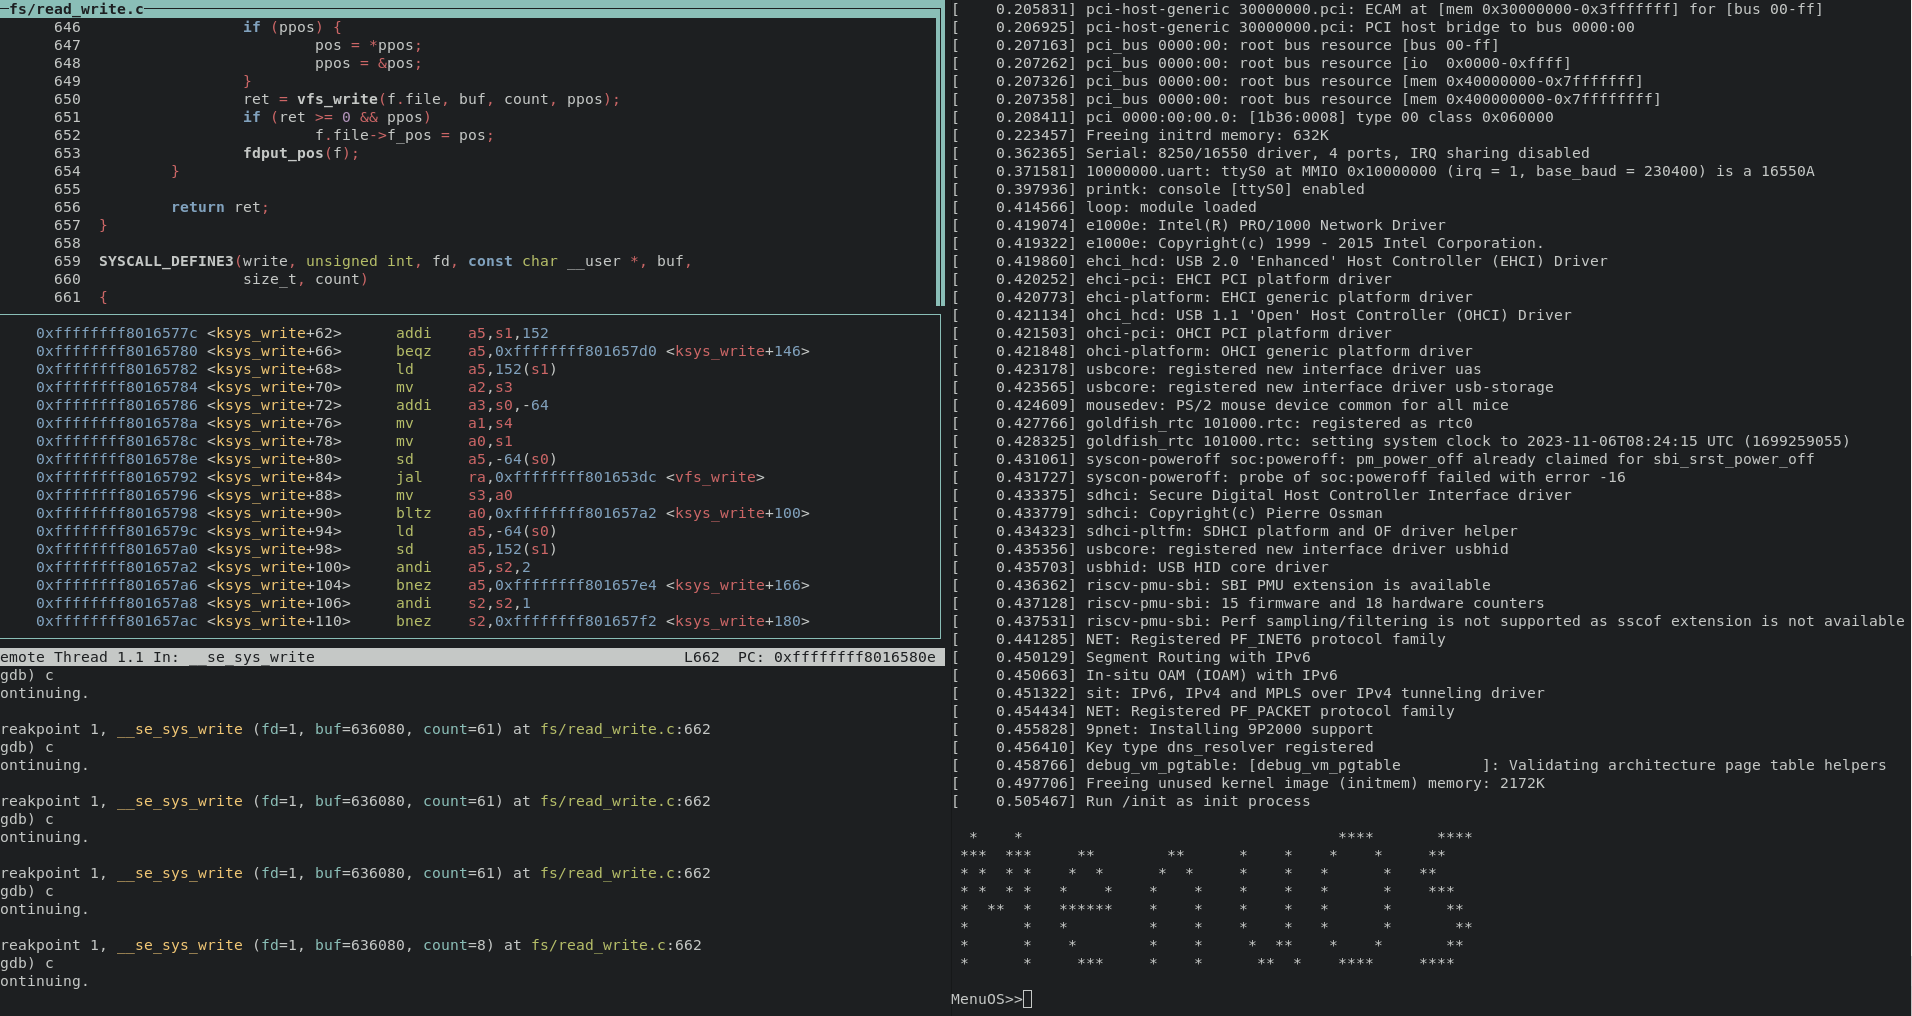
\includegraphics[width=0.7\textwidth]{image/image-20231106162535743.png}
  \caption{MenuOS加载shell}
\end{figure}

现在在MenuOS中输入  write-asm 回车之后, MenuOS将会暂停输出。然后在左侧gdb窗口中输入命令 c ,MenuOS将会显示以下信息:
\begin{figure}[htbp]
  \centering
  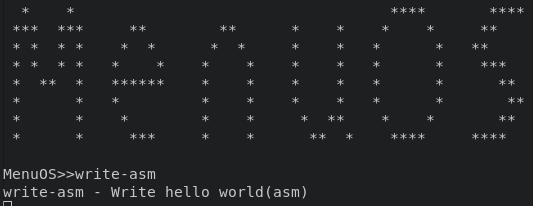
\includegraphics[width=0.7\textwidth]{image/image-20231106162854338.png}
  \caption{MenuOS运行write-asm}
\end{figure}

此时可以开始分析 Cwrite 中使用系统调用 write 的过程。首先使用以下命令对 handle\_exception 打断点:

\begin{lstlisting}
  b handle_exception
\end{lstlisting}

然后使用命令 c 进入到 handle\_exception 断点处。在 handle\_exception 函数中,根据异常号判断是否是系统调用。如果是系统调用,控制权会传递到系统调用处理的分发函数。
\begin{figure}[htbp]
  \centering
  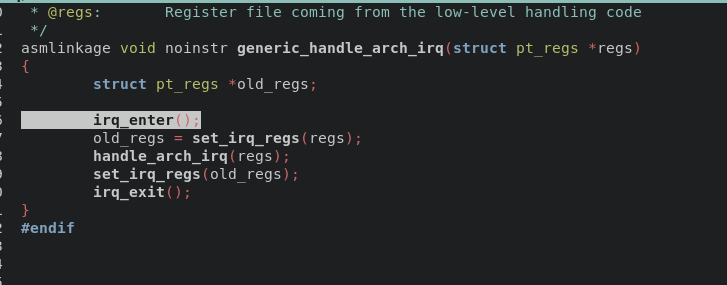
\includegraphics[width=0.7\textwidth]{image/image-20231111184909752.png}
  \caption{handle\_exception 断点处}
\end{figure}

generic\_handle\_arch\_irq 是 Linux 内核中的一个通用中断处理函数,它用于处理系统中断的基本工作。这个函数的主要作用是将控制权传递给适当的中断处理函数。在 Linux 内核中,每个中断都有一个对应的中断处理函数,用于处理特定类型的中断。generic\_handle\_arch\_irq 通过查询中断描述符表(Interrupt Descriptor Table,IDT)来确定要执行的中断处理函数,并将控制权转交给它。

使用命令 c 进入 ksys\_write 断点处。在 SYSCALL\_DEFINE3 的函数中的返回语句 return ksys\_write(fd, buf, count);  ,如下图所示:
\begin{figure}[htbp]
  \centering
  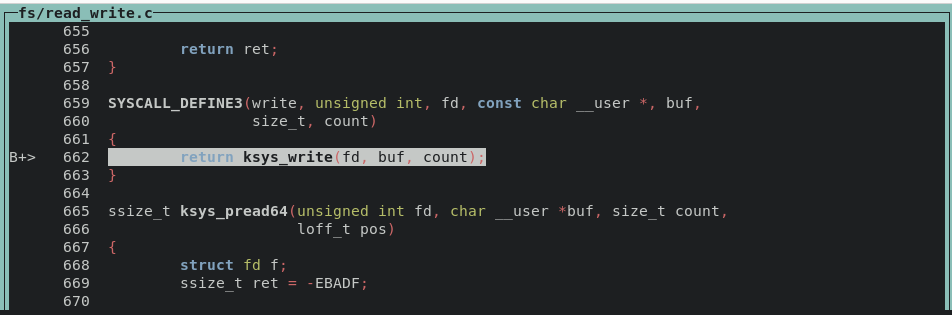
\includegraphics[width=0.7\textwidth]{image/image-20231106162942747.png}
  \caption{ksys\_write 断点处}
\end{figure}

继续使用 si 命令,将程序将执行下一条汇编语句,如下图所示:
\begin{figure}[htbp]
  \centering
  \includegraphics[width=0.7\textwidth]{image/image-20231106163210213.png}
  \caption{执行下一条汇编语句}
\end{figure}

system\_call 调用过程如下:
\begin{figure}[htbp]
  \centering
  \includegraphics[width=0.25\textwidth]{image/system\_call.png}
  \caption{system\_call 调用过程}
\end{figure}

\newpage
具体的流程
由于一些限制,光靠这个gdb无法明确的知道系统调用的一些细节,在这里展开讲解一些。

ecall触发trap,ecall它其实是跳转到一个地址,这个地址被存在stvec寄存器中(请了解RISCV特权架构指令)
这个stvec的地址在操作系统的启动的时候就已经被设置好了在arch/riscv/kernel/head.S 里面,它就是handle\_exception。
handle\_execption会保存用户的上下文,然后把内核上下文写入寄存器(包括页表)
sstatuc、sepc、stval、scause、sscratch 这 5 个 csr 寄存器(请了解RISCV特权架构指令)存储了触发trap的信息。
scause里面存储的是出发trap的信息,scause 寄存器最高位含义如下:最高位=1:interrupts 最高位=0:exceptions,如scause的值大于0那么就是由excptions触发,如果小于0,那么就是一个中断。我们这里是大于0的。

接下里判断scause是否等于EXC\_SYSCALL 这个值是8 ,也就是当 scause==8 时,就表示由 sys\_call 触发的 trap,从而进入handle\_syscall
handle\_syscall 里面会将spec也就是出错的地址(我们这里是ecall的地址)+4并且存储下来,用于正确返回(sret的时候是ret到下一个ecall的地址防止无限循环),然后根据a7里面的值确定是哪个系统调用。找到相应的系统调用,返回。注意在 handle\_syscall 里跳转到实际的系统调用函数时把返回地址设置成了 ret\_from\_syscall。所以上述的 sys\_write 函数返回后会跳转到 ret\_from\_syscall 继续执行。
ret\_from\_syscall会将保存的用户模式的上下文中的a0(返回值)切换为系统调用运行之后的返回值,然后恢复现场,最后使用sret来回到用户态


\chapter{实验六:分析 Linux 内核创建一个新进程的过程}

\begin{introduction}[实验要求:]
\item 阅读理解 task\_struct 数据结构 ;
\item 分析 fork 函数对应的内核处理过程 sys\_clone,理解创建一个新进程如何创建和修改 task\_struct 数据结构;
\item 使用 gdb 跟踪分析一个 fork 系统调用内核处理函数 sys\_clone
\item 验证对 Linux 系统创建一个新进程的理解. 特别关注新进程是从哪里开始执行的?为什么从那里能顺利执行下去?即执行起点与内核堆栈如何保证一致。  
\end{introduction}



\section{阅读理解 task\_struct 数据结构}
struct task\_struct结构体是用于描述进程的结构体。它非常庞大,其中列举几个常用的结构体成员以及用途:

\begin{itemize}
  \item thread\_info 描述进程的底层信息
  \item mm\_struct 指向内存区域描述符的指针
  \item tty\_struct 描述进程相关的tty设备
  \item pid 是进程的标识符
  \item fs\_struct 表示当前目录
  \item state 是进程状态
  \item files\_struct 指向文件描述符的指针
  \item stack 是堆栈
  \item thread 用于保存上下文中 CPU 相关状态信息的关键数据
  \item signal\_struct 表示接收到的信号
\end{itemize}

\section{分析 fork 函数对应的内核处理过程 sys\_clone}
对于 RISC-V Linux 系统来说,用户态程序执行 ecall 指令出发 entry\_SYSCALL64 并以 ret 返回系统调用。系统调用陷入内核态,用用户态堆栈转换到内核态堆栈。

fork 系统调用创建了一个子进程,子进程复制了父进程中所有的信息,包括内核堆栈、进程描述符等。fork 系统调用在内核里面变成了父、子两个进程,父进程正常fork系统调用返回用户态,子进程也要从内核态返回用户态。

在 RISC-V Linux 系统中没有定义 fork 系统调用,只在include/uapi/asm-generic/unistd.h定义了 clone 系统调用, 对于的内核处理函数为220号系统调用 sys\_clone。

\begin{figure}[htbp]
  \centering
  \includegraphics[width=0.6\textwidth]{image/image-20231107202345288.png}
  \caption{系统调用 sys\_clone}
\end{figure}


在Linux 5.19.16中这些创建进程的系统调用都是在kernel/fork, 文件中实现的,代码如下:

\begin{lstlisting}
pid_t kernel_clone(struct kernel_clone_args *args)
{
	u64 clone_flags = args->flags;
	struct completion vfork;
	struct pid *pid;
	struct task_struct *p; //待创建进程的进程描述符
	int trace = 0;
	pid_t nr; //待创建进程的pid

	if ((args->flags & CLONE_PIDFD) &&
	    (args->flags & CLONE_PARENT_SETTID) &&
	    (args->pidfd == args->parent_tid))
		return -EINVAL;

	if (!(clone_flags & CLONE_UNTRACED)) {
		if (clone_flags & CLONE_VFORK)
			trace = PTRACE_EVENT_VFORK;
		else if (args->exit_signal != SIGCHLD)
			trace = PTRACE_EVENT_CLONE;
		else
			trace = PTRACE_EVENT_FORK;

		if (likely(!ptrace_event_enabled(current, trace)))
			trace = 0;
	}

    //复制进程描述符和执行时所需的其他数据结构
	p = copy_process(NULL, trace, NUMA_NO_NODE, args);
	add_latent_entropy();

	if (IS_ERR(p))
		return PTR_ERR(p);

	trace_sched_process_fork(current, p);

	pid = get_task_pid(p, PIDTYPE_PID);
	nr = pid_vnr(pid);

	if (clone_flags & CLONE_PARENT_SETTID)
		put_user(nr, args->parent_tid);

	if (clone_flags & CLONE_VFORK) {
		p->vfork_done = &vfork;
		init_completion(&vfork);
		get_task_struct(p);
	}

	wake_up_new_task(p);//将子进程添加到就绪队列,使之有机会被调度执行

	/* forking complete and child started to run, tell ptracer */
	if (unlikely(trace))
		ptrace_event_pid(trace, pid);

	if (clone_flags & CLONE_VFORK) {
		if (!wait_for_vfork_done(p, &vfork))
			ptrace_event_pid(PTRACE_EVENT_VFORK_DONE, pid);
	}

	put_pid(pid);
	return nr;
}


pid_t kernel_thread(int (*fn)(void *), void *arg, unsigned long flags)
{
	struct kernel_clone_args args = {
		.flags		= ((lower_32_bits(flags) | CLONE_VM |
				    CLONE_UNTRACED) & ~CSIGNAL),
		.exit_signal	= (lower_32_bits(flags) & CSIGNAL),
		.fn		= fn,
		.fn_arg		= arg,
		.kthread	= 1,
	};

	return kernel_clone(&args);
}


pid_t user_mode_thread(int (*fn)(void *), void *arg, unsigned long flags)
{
	struct kernel_clone_args args = {
		.flags		= ((lower_32_bits(flags) | CLONE_VM |
				    CLONE_UNTRACED) & ~CSIGNAL),
		.exit_signal	= (lower_32_bits(flags) & CSIGNAL),
		.fn		= fn,
		.fn_arg		= arg,
	};

	return kernel_clone(&args);
}

#ifdef __ARCH_WANT_SYS_FORK
SYSCALL_DEFINE0(fork)
{
#ifdef CONFIG_MMU
	struct kernel_clone_args args = {
		.exit_signal = SIGCHLD,
	};

	return kernel_clone(&args);
#else
	/* can not support in nommu mode */
	return -EINVAL;
#endif
}
#endif

#ifdef __ARCH_WANT_SYS_VFORK
SYSCALL_DEFINE0(vfork)
{
	struct kernel_clone_args args = {
		.flags		= CLONE_VFORK | CLONE_VM,
		.exit_signal	= SIGCHLD,
	};

	return kernel_clone(&args);
}
#endif                                     

#ifdef __ARCH_WANT_SYS_CLONE
#ifdef CONFIG_CLONE_BACKWARDS
SYSCALL_DEFINE5(clone, unsigned long, clone_flags, unsigned long, newsp,
		 int __user *, parent_tidptr,
		 unsigned long, tls,
		 int __user *, child_tidptr)
#elif defined(CONFIG_CLONE_BACKWARDS2)

\end{lstlisting}
从上面的代码可以看出,fork、vfork和clone这三个系统调用以及user\_mode\_thread和kernel\_thread内核函数都能创建一个新的进程,而且都是通过kernel\_clone这个函数来创建的,只是传递的参数不一样。

理解创建一个新进程如何创建和修改 task\_struct 数据结构
创建一个进程是复制当前进程的信息,通过kernel\_clone函数创建一个新的进程。因为父进程和子进程的绝大部分信息是一样的,除开pid的值和内核堆栈以及thread结构体变量记录进程执行上下文的CPU关键信息。

kernel\_clone的代码如下:
\begin{lstlisting}
pid_t kernel_clone(struct kernel_clone_args *args)
{
	u64 clone_flags = args->flags;
	struct completion vfork;
	struct pid *pid;
	struct task_struct *p; //待创建进程的进程描述符
	int trace = 0;
	pid_t nr; //待创建进程的pid

	if ((args->flags & CLONE_PIDFD) &&
	    (args->flags & CLONE_PARENT_SETTID) &&
	    (args->pidfd == args->parent_tid))
		return -EINVAL;

	if (!(clone_flags & CLONE_UNTRACED)) {
		if (clone_flags & CLONE_VFORK)
			trace = PTRACE_EVENT_VFORK;
		else if (args->exit_signal != SIGCHLD)
			trace = PTRACE_EVENT_CLONE;
		else
			trace = PTRACE_EVENT_FORK;

		if (likely(!ptrace_event_enabled(current, trace)))
			trace = 0;
	}

        //复制进程描述符和执行时所需的其他数据结构
	p = copy_process(NULL, trace, NUMA_NO_NODE, args);
	add_latent_entropy();

	if (IS_ERR(p))
		return PTR_ERR(p);

	trace_sched_process_fork(current, p);

	pid = get_task_pid(p, PIDTYPE_PID);
	nr = pid_vnr(pid);

	if (clone_flags & CLONE_PARENT_SETTID)
		put_user(nr, args->parent_tid);

	if (clone_flags & CLONE_VFORK) {
		p->vfork_done = &vfork;
		init_completion(&vfork);
		get_task_struct(p);
	}

	wake_up_new_task(p);//将子进程添加到就绪队列,使之有机会被调度执行

	/* forking complete and child started to run, tell ptracer */
	if (unlikely(trace))
		ptrace_event_pid(trace, pid);

	if (clone_flags & CLONE_VFORK) {
		if (!wait_for_vfork_done(p, &vfork))
			ptrace_event_pid(PTRACE_EVENT_VFORK_DONE, pid);
	}
	put_pid(pid);
	return nr;
}

\end{lstlisting}
从这段代码可以看出创建一个新进程的流程如下:
\begin{figure}[htbp]
  \centering
  \includegraphics[width=0.25\textwidth]{image/fork.png}
  \caption{创建一个新进程}
\end{figure}

而对于创建一个新进程进而修改 task\_struct 数据结构的秘密就在获取父进程的进程描述符和其他数据结构的步骤之中,涉及的函数就是 copy\_process()。限于篇幅,现在简短的讲解 copy\_process() 的内容。

copy\_process() 函数主要是做了以下几件事情:

\begin{enumerate}
  \item 复制进程描述符task\_struct、创建内核堆栈
  \item 复制所有的进程信息
  \item 初始化子进程和thread
  \item 为子进程分配新的pid
  \item 增加系统中的进程数目
  \item 返回被创建的子进程描述符指针
\end{enumerate}

而第一件事情——复制进程描述符task\_struct、创建内核堆栈,调用了 dup\_task\_struct 函数,而这个函数是实际复制进程描述符的关键函数。

\section{GDB 跟踪分析sys\_clone}
使用 gdb 跟踪分析一个 fork 系统调用内核处理函数 sys\_clone,我们在menuos中的test.c文件中的添加了ForkProcess函数,内容如下:

\begin{lstlisting}
int ForkProcess(int argc, char *argv[]){
  int pid;
  pid = fork();
  if(pid < 0){
    fprintf(stderr, "Fork Failed!");
    exit(-1);
  }
  else if (pid == 0){
    printf("This is Child Process!\n");
  }
  else {
    printf("This is Parent Process!\n");
    wait(NULL);
    printf("Child Complete!\n");
  }
}
\end{lstlisting}
并在main函数中添加以下语句:

\begin{lstlisting}
  MenuConfig("fork-new", "fork new process", ForkProcess);
\end{lstlisting}

在menuos的目录下使用以下命令启动 qemu 模拟 riscv 架构同时启动gdbserver:

\begin{lstlisting}
  ./init-gdb.sh
\end{lstlisting}

新建另一个shell在menuos目录中输入以下命令,启动 gdb-multiarch 并加载Linux内核符号表:

\begin{lstlisting}
  ./start-gdb.sh
\end{lstlisting}

然后依次打入 sys\_clone 、 kernel\_clone 、 dup\_task\_struct 、 copy\_process 、copy\_thread 、 ret\_from\_fork 的断点。
\begin{figure}[htbp]
  \centering
  \includegraphics[width=0.7\textwidth]{image/image-20231107213842226.png}
  \caption{打入断点}
\end{figure}

从上图中可以发现 do\_fork 这个函数的确已经在5.19.16的内核删除,并使用kernel\_clone代替了。

\newpage
待程序成功加载Menuos后,在MenuOS中输入 fork-new 使用 ForkProcess 函数创建新的进程。
\begin{figure}[htbp]
  \centering
  \includegraphics[width=0.7\textwidth]{image/image-20231107214310340.png}
  \caption{fork-new}
\end{figure}

首先启动的是\_\_se\_sys\_clone,如下图所示:
\begin{figure}[htbp]
  \centering
  \includegraphics[width=0.7\textwidth]{image/image-20231107215732335.png}
  \caption{\_\_se\_sys\_clone}
\end{figure}

然后启动的是kernel\_clone:
\begin{figure}[htbp]
  \centering
  \includegraphics[width=0.7\textwidth]{image/image-20231107215834035.png}
  \caption{\_\_se\_sys\_clone}
\end{figure}

\newpage
接着是copy\_process:
\begin{figure}[htbp]
  \centering
  \includegraphics[width=0.7\textwidth]{image/image-20231107215857474.png}
  \caption{copy\_process}
\end{figure}

然后开始复制所有的进程信息
\begin{figure}[htbp]
  \centering
  \includegraphics[width=0.7\textwidth]{image/image-20231107214335881.png}
  \caption{复制所有的进程信息}
\end{figure}

接着进入copy\_thread
\begin{figure}[htbp]
  \centering
  \includegraphics[width=0.7\textwidth]{image/image-20231107214346193.png}
  \caption{copy\_thread}
\end{figure}


最后返回子进程
\begin{figure}[htbp]
  \centering
  \includegraphics[width=0.7\textwidth]{image/image-20231107214357751.png}
  \caption{返回子进程}
\end{figure}

\newpage
MenuOS上如下:
\begin{figure}[htbp]
  \centering
  \includegraphics[width=0.7\textwidth]{image/image-20231107214407872.png}
  \caption{MenuOS}
\end{figure}


本次调试过程基本符合之前分析的步骤。

\chapter{实验七:Linux 内核如何装载和启动一个可执行程}

\begin{introduction}[实验要求:]
\item 理解编译链接的过程和 ELF 可执行文件格式
\item 编程使用 exec库函数加载一个可执行文件,动态链接分为可执行程序装载时动态链接和运行时动态链接,编程练习动态链接库的这两种使用方式
\item 使用 gdb 跟踪分析一个 execve 系统调用内核处理函数 sys\_execve
\item 验证对 Linux 系统加载可执行程序所需处理过程的理解。特别关注新的可执行程序是从哪里开始执行的?
\item 为什么 execve 系统调用返回后新的可执行程序能顺利执行?对于静态链接的可执行程序和动态链接的可执行程序 execve 系统调用返回时会有什么不同?
\end{introduction}

\section{程序的编译过程}
程序从源代码到可执行文件的编译步骤分为4步:
\begin{figure}[htbp]
  \centering
  \includegraphics[width=0.1\textwidth]{image/execve.png}
  \caption{编译过程}
\end{figure}


在预处理过程中,主要是完成删除和展开以及处理命令这三种操作,最后将文本保存到后缀为 .i 文件中。以预处理 hello.c 文件为例。

下面是 hello.c 文件的内容:
\begin{lstlisting}
  #include <stdio.h>
  
  void main(){
    printf("hello world!\n");
  }  
\end{lstlisting}

使用ssh 连接好 visionfive 2 开发板后,使用vim创建 hello.c 文件。

然后执行以下的预处理命令得到 hello.i 文件:

\begin{lstlisting}
  gcc -E hello.c -o hello.i
\end{lstlisting}

使用 vim 打开 hello.i 文件后内容较多,但可以看出有几大特点:

首先是 \#include 命令全部替换成包含文件的路径,如下图所示:
\begin{figure}[htbp]
  \centering
  \includegraphics[width=0.7\textwidth]{image/image-20231108152215370.png}
  \caption{ \#include 替换}
\end{figure}


同时添加了行号和文件名标示:
\begin{figure}[htbp]
  \centering
  \includegraphics[width=0.4\textwidth]{image/image-20231108152332267.png}
  \caption{添加标示}
\end{figure}


其次是删除了所有的注释。

编译是在预处理的基础上,gcc首先检查代码的规范性和语法错误,检查无误后的翻译为汇编语言。

使用以下的命令将预处理的中的代码生成为汇编语言代码:

\begin{lstlisting}
  gcc -S hello.i -o hello.s
\end{lstlisting}

以下的在 visionfive 2 中编译完的RISCV架构的汇编代码:

\begin{lstlisting}
  .file	"hello.c"
  .option pic
  .attribute arch, "rv64i2p1_m2p0_a2p1_f2p2_d2p2_c2p0_zicsr2p0_zifencei2p0"
  .attribute unaligned_access, 0
  .attribute stack_align, 16
  .text
  .section	.rodata
  .align	3
  .LC0:
  .string	"Hello world!"
  .text
  .align	1
  .globl	main
  .type	main, @function
  main:
  addi	sp,sp,-16
  sd	ra,8(sp)
  sd	s0,0(sp)
  addi	s0,sp,16
  lla	a0,.LC0
  call	puts@plt
  nop
  ld	ra,8(sp)
  ld	s0,0(sp)
  addi	sp,sp,16
  jr	ra
  .size	main, .-main
  .ident	"GCC: (Debian 12.2.0-10) 12.2.0"
  .section	.note.GNU-stack,"",@progbits
\end{lstlisting}
链接就是将各个代码和数据收集起来组合成一个单一文件的过程。以下的命令将生成RISC-V Linux下的可执行文件:

\begin{lstlisting}
  gcc hello.o -o hello -static
\end{lstlisting}
以下是节表头:

\begin{lstlisting}
  There are 28 section headers, starting at offset 0x7a490:

  Section Headers:
  [Nr] Name              Type             Address           Offset
  Size              EntSize          Flags  Link  Info  Align
  [ 0]                   NULL             0000000000000000  00000000
  0000000000000000  0000000000000000           0     0     0
  [ 1] .note.gnu.bu[...] NOTE             00000000000101c8  000001c8
  0000000000000024  0000000000000000   A       0     0     4
  [ 2] .note.ABI-tag     NOTE             00000000000101ec  000001ec
  0000000000000020  0000000000000000   A       0     0     4
  [ 3] .rela.dyn         RELA             0000000000010210  00000210
  0000000000000210  0000000000000018   A      25     0     8
  [ 4] .text             PROGBITS         0000000000010420  00000420
  00000000000412b2  0000000000000000  AX       0     0     4
  [ 5] __libc_freeres_fn PROGBITS         00000000000516d2  000416d2
  0000000000000814  0000000000000000  AX       0     0     2
  [ 6] .rodata           PROGBITS         0000000000051ef0  00041ef0
  000000000001b4a4  0000000000000000   A       0     0     16
\end{lstlisting}

编程使用 exec库函数加载一个可执行文件
在 visionfive 2 开发板上启动debain后,使用以下的命令使用man命令查看execve函数信息:

\begin{lstlisting}
  man execve
\end{lstlisting}

execve函数信息如下:
\begin{figure}[htbp]
  \centering
  \includegraphics[width=0.4\textwidth]{image/image-20231108204744069.png}
  \caption{execve函数信}
\end{figure}


现在编写一个叫作 local\_exec.c 的文件,使用 exec 系统调用加载之前编译产生的 hello 可执行文件。下面的是 local\_exec.c 的内容:

\begin{lstlisting}
  #include <stdio.h>
  #include <unistd.h>

  int main() {
    int pid;
    /* fork another process */
    pid = fork();
    if (pid < 0) 
    { 
      /* error occurred */
      fprintf(stderr,"Fork Failed!");
      exit(-1);
    } 
    else if (pid == 0) 
    {
      /*	 child process 	*/
      printf("This is Child Process!\n");
      execlp("/hello","hello",NULL);
    } 
    else 
    { 	
      /* 	parent process	 */
      printf("This is Parent Process!\n");
      /* parent will wait for the child to complete*/
      wait(NULL);
      printf("Child Complete!\n");
    }
  }
\end{lstlisting}
在 execl 函数中,第一个参数是可执行文件的路径,第二个参数是程序的名称,最后一个参数必须是 (char *)0。

使用以下命令进行编译:

\begin{lstlisting}
  gcc -o local_exec local_exec.c
\end{lstlisting}

运行结果如下:
\begin{figure}[htbp]
  \centering
  \includegraphics[width=0.7\textwidth]{image/image-20231109161948754.png}
  \caption{local\_exec}
\end{figure}


\section{动态链接}
动态链接是一种在程序运行时将代码和数据与程序链接的技术,而不是在编译时将它们链接到可执行文件中。它提供了灵活性和共享性,允许多个程序共享和重复使用相同的库代码。动态链接主要分为两种方式:可执行程序装载时动态链接和运行时动态链接。相比于静态链接,动态链接可以多个程序共享同一个段代码,而不需要多个副本。但是动态链接对库的依赖程度高。

可执行程序装载时动态链接是指动态链接发生在可执行程序被加载到内存时查找和链接动态链接库。运行时动态链接是指程序在运行时显式加载并链接动态链接库,然后调用库中的函数。

可执行程序装载时动态链接通常更加高效,因为它减少了运行时的开销,而运行时动态链接提供了更大的灵活性,允许动态加载和卸载库,以便在运行时进行插件或模块式的扩展。

gcc默认编译就是动态链接,使用以下命令动态链接 hello 可执行文件:

\begin{lstlisting}
  gcc hello.o -o hello.dynamic
\end{lstlisting}

使用  ls -l 命令可以发现在RISC-V架构下动态链接的可执行文件比静态链接的可执行文件小58倍,而书上比较x86的比值是100倍:
\begin{figure}[htbp]
  \centering
  \includegraphics[width=0.7\textwidth]{image/image-20231108210901120.png}
  \caption{文件大小比较}
\end{figure}

以下是用于实践动态链接的代码:

首先是可执行程序装载时动态链接代码,我们需要创建两个文件,分别是 shlibexample.h 和 shlibexample.c 文件。

shlibexample.h 源代码如下:


\begin{lstlisting}
  #ifndef _SH_LIB_EXAMPLE_H_
  #define _SH_LIB_EXAMPLE_H_

  #define SUCCESS 0
  #define FAILURE (-1)

  #ifdef __cplusplus
  extern "C"{
    #endif
    int SharedLibApi();
    #ifdef __cplusplus
  }
  #endif
  #endif
\end{lstlisting}

shlibexample.c  源代码如下:

\begin{lstlisting}
  #include <stdio.h>
  #include "shlibexample.h"

  int SharedLibApi(){
    printf("This is a shared library!\n");
    return SUCCESS;
  }
\end{lstlisting}
保存好后文件后,在visionfive 2 开发板使用以下命令,创建 libshlibexample.so 文件:

\begin{lstlisting}
  gcc -shared shlibexample.c -o libshlibexample.so
\end{lstlisting}
实现运行时动态链接,我们也需要创建两个文件,分别是 dllibexample.h 和 dllibexample.c 文件。

dllibexample.h 源代码如下:

\begin{lstlisting}
  #ifndef _DL_LIB_EXAMPLE_H_
  #define _DL_LIB_EXAMPLE_H_

  #ifdef __cplusplus
  extern "C"{
    #endif
    
    int DynamicalLoadingLibAPi();
    
    #ifdef __cplusplus
  }
  #endif
  #endif
\end{lstlisting}
dllibexample.c 源代码如下:

\begin{lstlisting}
  #include <stdio.h>
  #include "dllibexample.h"

  #define SUCCESS 0
  #define FAILURE (-1)

  int DynamicalLoadingLibAPi(){
    printf("This is a Dynamical Loading library!\n");
    return SUCCESS;
  }
\end{lstlisting}
同样保存好后文件后,在visionfive 2 开发板使用以下命令,创建 libdlibexample.so 文件:

\begin{lstlisting}
  gcc -shared dllibexample.c -o libdlibexample.so
\end{lstlisting}

当分别生成好 libshlibexample.so 文件和 libdlibexample.so 文件后,我们需要分别调用这两个文件。在visionfive 2 开发板中创建一个名为 main.c 的文件,main.c 的内容如下:

\begin{lstlisting}
  #include <stdio.h>
  #include "shlibexample.h"
  #include <dlfcn.h>

  int main(){
    printf("Calling SharedLibApi() function of libshlibexample.so!\n");
    SharedLibApi();
    
    void * handle = dlopen("libdlibexample.so", RTLD_NOW);
    if(handle == NULL){
      printf("Open Lib libdllibexample.so Error:%s\n", dlerror());
      return FAILURE;
    }
    int (*func)(void);
    char *error;
    func = dlsym(handle ,"DynamicalLoadingLibAPi");
    if((error = dlerror()) != NULL){
      printf("DynamicalLoadingLibAPi() not found:%s\n", error);
      return FAILURE;
    }
    printf("Calling DynamicalLoadingLibApi() function of libdlibexample.so!\n");
    func();
    dlclose(handle);
    return SUCCESS;
  }
\end{lstlisting}

编辑好保存后,使用以下命令编译成 main 可执行文件:

\begin{lstlisting}
  gcc main.c -o main -L/root/Code/ -lshlibexample -ldl
\end{lstlisting}

然后将之前生成的 shlibexample.so 文件拷贝到 /usr/local/lib 中否则程序无法找到 shlibexample.so文件。完成以上工作后,使用以下命令,即可实现可执行程序装载时动态链接和运行时动态链接:

\begin{lstlisting}
  ./main	
\end{lstlisting}
成功运行后,会显示以下信息:
\begin{figure}[htbp]
  \centering
  \includegraphics[width=0.7\textwidth]{image/image-20231108220153906.png}
  \caption{可执行程序装载时动态链接和运行时动态链接}
\end{figure}



\section{gdb 跟踪分析一个 execve 系统调用}
进入MenuOS目录中的menuos目录后,编辑test.c, 在其中加入以下代码:

首先添加以下的头文件

\begin{lstlisting}
  #include <unistd.h>
\end{lstlisting}
然后添加 Exec 函数:


\begin{lstlisting}
  int Exec(int argc, char *argv[])
  {
    int pid;
    /* fork another process */
    pid = fork();
    if (pid < 0)
    {
      /* error occurred */
      fprintf(stderr,"Fork Failed!");
      exit(-1);
    }
    else if (pid == 0)
    {
      /*	 child process 	*/
      printf("This is Child Process!\n");
      execlp("/hello","hello",NULL);
    }
    else
    {
      /* 	parent process	 */
      printf("This is Parent Process!\n");
      /* parent will wait for the child to complete*/
      wait(NULL);
      printf("Child Complete!\n");
    }
  }
\end{lstlisting}
最后在 main 函数中添加以下语句:

\begin{lstlisting}
  MenuConfig("execve", "execve new process", Exec);
\end{lstlisting}
在menuos目录下使用以下语句进行编译:

\begin{lstlisting}
  make
  make rootfs
\end{lstlisting}
编译完成后,在两个终端上分别启动 init-gdb.sh 和 start-gdb.sh 脚本。脚本启动后,在启动 start-gdb.sh 的终端上输入 target remote:1234 连接qemu中的gdbserver。完成后,使用下述命令在gdb中为 sys\_execve 设置断点:


\begin{lstlisting}
  b sys_execve
\end{lstlisting}

\newpage
打好断点后,使用 c 命令,加载MenuOS后输入 exec 开始调试 exec,如下图所示:
\begin{figure}[htbp]
  \centering
  \includegraphics[width=0.7\textwidth]{image/image-20231109163507762.png}
  \caption{调试 exec}
\end{figure}


首先跳转到 SYSCALL\_DEFINE3(execve, ....) :
\begin{figure}[htbp]
  \centering
  \includegraphics[width=0.7\textwidth]{image/image-20231109164518819.png}
  \caption{SYSCALL\_DEFINE3}
\end{figure}


函数体中有 do\_execve()  ,然后使用 b do\_execve 命令进行打断点:
\begin{figure}[htbp]
  \centering
  \includegraphics[width=0.7\textwidth]{image/image-20231109165602046.png}
  \caption{b do\_execve }
\end{figure}

\newpage
进入 do\_execve()  后调用 do\_execveat\_common 函数, 现在给do\_execveat\_common 函数打上断点:
\begin{figure}[htbp]
  \centering
  \includegraphics[width=0.7\textwidth]{image/image-20231109165917824.png}
  \caption{b do\_execveat\_common }
\end{figure}


而大部分的工作基本上都是在 do\_execveat\_common 函数内完成的,do\_execveat\_common 函数执行完后会依次返回到 SYSCALL\_DEFINE3(execve, ....)  中完成调用, 完成调用后 MenuOS中的Shell将显示 hello world!:
\begin{figure}[htbp]
  \centering
  \includegraphics[width=0.7\textwidth]{image/image-20231109165138037.png}
  \caption{hello world!}
\end{figure}


但此时,进程仍然没有结束,下一步将进入 schedule 函数中依次执行 schedule 函数中的内容:
\begin{figure}[htbp]
  \centering
  \includegraphics[width=0.7\textwidth]{image/image-20231109164729388.png}
  \caption{schedule}
\end{figure}

\newpage
schedule 函数结束后,将再次引发 Shell 程序引起的中断:
\begin{figure}[htbp]
  \centering
  \includegraphics[width=0.7\textwidth]{image/image-20231109170505625.png}
  \caption{Shell 程序中断}
\end{figure}

此时MenuOS中的Shell可以再次输入命令。

\chapter{实验八:理解进程调度时机跟踪分析进程调度与进程切换的过程}
\begin{introduction}[实验要求]
\item 理解 Linux 系统中进程调度的时机
\item 使用 gdb 跟踪分析一个 schedule()函数
\item 仔细分析 switch\_to 中的汇编代码,理解进程上下文的切换机制,以及与中断上下文切换的关系;
\end{introduction}

\section{理解 Linux 系统中进程调度的时机}
进程是计算机中运行的程序的抽象,它包含了程序代码、数据、以及程序执行的上下文。进程调度的策略和算法决定哪个进程应该在某个时刻运行。进程调度的时机大多和中断有关。在多任务操作系统中,中断是一种机制,它允许操作系统在发生某些事件时打断正在执行的进程,转而执行另一个进程。这种打断和切换的机制是进程调度的基础——中断上下文恢复。中断上下文恢复是指在中断服务例程(ISR)中,由于中断事件而中断的正在执行的任务(通常是用户进程)的上下文(包括寄存器状态、程序计数器等)被保存起来,以便在中断处理完成后能够正确地恢复原来的任务继续执行。

\section{gdb 跟踪分析 schedule()函数}
在menuos的目录之下,启动 init\_gdb.sh 和 star-gdb.sh 两个bash脚本和gdb远程连接后,在gdb中输入 b schedule 命令进行对schedule函数进行打断点后,使用c 命令运行到断点处。如下图所示:
\begin{figure}[htbp]
  \centering
  \includegraphics[width=0.7\textwidth]{image/image-20231109201036323.png}
  \caption{gdb schedule}
\end{figure}

在RISC-V架构下的Linux内核中,schedule断点并没有出现在 kernel/sched/core.c 中而是出现在 arch/riscv/include/asm/current.h 中,并指向 riscv\_current\_is\_tp 。
\begin{figure}[htbp]
  \centering
  \includegraphics[width=0.7\textwidth]{image/image-20231109201842239.png}
  \caption{riscv\_current\_is\_tp}
\end{figure}

\newpage
在进行下一步后,断点跳至 kernel/sched/core.c 中的 schedule 函数中:
\begin{figure}[htbp]
  \centering
  \includegraphics[width=0.7\textwidth]{image/image-20231109202045031.png}
  \caption{jump to schedule}
\end{figure}


\newpage
在 tsk 变量赋值后, 使用 p *tsk 命令查看 tsk 的内容:
\begin{figure}[htbp]
  \centering
  \includegraphics[width=0.7\textwidth]{image/image-20231109202345331.png}
  \caption{p *tsk}
\end{figure}


使用 b \_\_schedule 对 \_\_schedule 设置断点并使用 c 命令运行到断点处:
\begin{figure}[htbp]
  \centering
  \includegraphics[width=0.7\textwidth]{image/image-20231109202607880.png}
  \caption{b \_\_schedule}
\end{figure}


\newpage
在 \_\_schedule 函数中使用 n 命令单独后,发现 \_\_schedule 函数调用了 context\_switch 函数:
\begin{figure}[htbp]
  \centering
  \includegraphics[width=0.7\textwidth]{image/image-20231109202816225.png}
  \caption{调用 context\_switch 函数}
\end{figure}


\newpage
对 context\_switch 打入断点后,单步执行后发现调用 switch\_to:
\begin{figure}[htbp]
  \centering
  \includegraphics[width=0.7\textwidth]{image/image-20231109203216397.png}
  \caption{调用 switch\_to}
\end{figure}


此时无法对 switch\_to  进行打断点,因为 switch-to 是一个宏定义,在预处理阶段就已经被替换了,所以只能对 \_\_switch\_to 打断点,由于RISC-V架构下 \_\_switch\_to 是有纯汇编写的,所以无法展示c语言代码。如下图所示:
\begin{figure}[htbp]
  \centering
  \includegraphics[width=0.7\textwidth]{image/image-20231109204506752.png}
  \caption{b \_\_switch\_to}
\end{figure}


\section{分析 switch\_to 中的汇编代码}
在RISC-V架构的Linux内核中,switch\_to的汇编代码位于 arch/riscv/kernel/entry.S 中。

以下代码是switch\_to部分的汇编代码:

\begin{lstlisting}
  ENTRY(__switch_to)
  /* Save context into prev->thread */
  li    a4,  TASK_THREAD_RA
  add   a3, a0, a4
  add   a4, a1, a4
  REG_S ra,  TASK_THREAD_RA_RA(a3)
  REG_S sp,  TASK_THREAD_SP_RA(a3)
  REG_S s0,  TASK_THREAD_S0_RA(a3)
  REG_S s1,  TASK_THREAD_S1_RA(a3)
  REG_S s2,  TASK_THREAD_S2_RA(a3)
  REG_S s3,  TASK_THREAD_S3_RA(a3)
  REG_S s4,  TASK_THREAD_S4_RA(a3)
  REG_S s5,  TASK_THREAD_S5_RA(a3)
  REG_S s6,  TASK_THREAD_S6_RA(a3)
  REG_S s7,  TASK_THREAD_S7_RA(a3)
  REG_S s8,  TASK_THREAD_S8_RA(a3)
  REG_S s9,  TASK_THREAD_S9_RA(a3)
  REG_S s10, TASK_THREAD_S10_RA(a3)
  REG_S s11, TASK_THREAD_S11_RA(a3)
  /* Restore context from next->thread */
  REG_L ra,  TASK_THREAD_RA_RA(a4)
  REG_L sp,  TASK_THREAD_SP_RA(a4)
  REG_L s0,  TASK_THREAD_S0_RA(a4)
  REG_L s1,  TASK_THREAD_S1_RA(a4)
  REG_L s2,  TASK_THREAD_S2_RA(a4)
  REG_L s3,  TASK_THREAD_S3_RA(a4)
  REG_L s4,  TASK_THREAD_S4_RA(a4)
  REG_L s5,  TASK_THREAD_S5_RA(a4)
  REG_L s6,  TASK_THREAD_S6_RA(a4)
  REG_L s7,  TASK_THREAD_S7_RA(a4)
  REG_L s8,  TASK_THREAD_S8_RA(a4)
  REG_L s9,  TASK_THREAD_S9_RA(a4)
  REG_L s10, TASK_THREAD_S10_RA(a4)
  REG_L s11, TASK_THREAD_S11_RA(a4)
  /* The offset of thread_info in task_struct is zero. */
  move tp, a1
  ret
  ENDPROC(__switch_to)
\end{lstlisting}

\section{分析汇编代码}
看到这段汇编代码,我们首先要做的是预处理一下,首先理解这个REG...和TASH...这些宏是什么。这里可以通过全局搜索,找到他们的定义。经过全局搜索发现,他们被定义在arch/riscv/include/asm/include.h里面。

\begin{lstlisting}
  #ifndef _ASM_RISCV_ASM_H
  #define _ASM_RISCV_ASM_H

  #ifdef __ASSEMBLY__
  #define __ASM_STR(x)	x
  #else
  #define __ASM_STR(x)	#x
  #endif

  #if __riscv_xlen == 64
  #define __REG_SEL(a, b)	__ASM_STR(a)
  #elif __riscv_xlen == 32
  #define __REG_SEL(a, b)	__ASM_STR(b)
  #else
  #error "Unexpected __riscv_xlen"
  #endif

  #define REG_L		__REG_SEL(ld, lw)
  #define REG_S		__REG_SEL(sd, sw)
\end{lstlisting}


在riscv中一个字是32位,64字是double world。在汇编代码中一般用w(32位)表示一个字,用d(64位)表示2个字。在c语言的宏里面\#的作用是将传入的字符变成一个用双引号包裹的字符串(请自行查看相关标准)。我们这里不需要双引号,并且是64位,所以REG\_L预处理之后应该是ld和sd

在arch/riscv/kernel/asm-offsets.c中我们可以找到TASK\_THREAD\_RA\_RA的定义

\begin{lstlisting}
  void asm_offsets(void)
  {
    OFFSET(TASK_THREAD_RA, task_struct, thread.ra);
    ...
    DEFINE(TASK_THREAD_RA_RA,
    offsetof(struct task_struct, thread.ra)
    - offsetof(struct task_struct, thread.ra)
    );
  }
\end{lstlisting}
这个TASK\_THREAD\_RA\_RA的意思就是得到ra寄存器距离ra寄存器的offset。这里是用task\_struct里面的thread.ra的地址减去thrad.ra的地址。而TASH\_THREAD\_RA就是thread.ra距离task\_struct的偏移地址。
接下来我们来看看这个thread的数据结构,它在/arch/riscv/include/asm/processor.h里面。

\begin{lstlisting}
  struct thread_struct {
    /* Callee-saved registers */
    unsigned long ra;
    unsigned long sp;	/* Kernel mode stack */
    unsigned long s[12];	/* s[0]: frame pointer */
    struct __riscv_d_ext_state fstate;
    unsigned long bad_cause;
    unsigned long vstate_ctrl;
    struct __riscv_v_ext_state vstate;
  };
\end{lstlisting}
我们再来看看调用switch\_to的代码,发现第一个参数是需要保存的tash\_struct第二个参数是需要加载的tash\_struct。
也就是说a0 = prev ,a1 = next

\begin{lstlisting}
  #define switch_to(prev, next, last)		
  do {						
    struct task_struct *__prev = (prev);	
    struct task_struct *__next = (next);	
    if (has_fpu())				
    __switch_to_aux(__prev, __next);	
    ((last) = __switch_to(__prev, __next));	
  } while (0)
\end{lstlisting}
让我们以伪代码的形式来理解这段代码。

\begin{lstlisting}
  a0 = prev
  a1 = next 
  offset = &task_struct - &(task_struct->ra)//ra距离task_struct偏移
  ENTRY(__switch_to)
  /* Save context into prev->thread */
  li    a4,  offset
  add   a3, a0, a4 //a3 = prev->thread.ra
  add   a4, a1, a4 //a4 = next->thread.ra
  sd ra,  a3 
  sd sp,  8(a3)
  sd s0,  16(a3)
  sd s1,  24(a3)
  sd s2,  32(a3)
  sd s3,  40(a3)
  sd s4,  48(a3)
  sd s5,  56(a3)
  sd s6,  64(a3)
  sd s7,  72(a3)
  sd s8,  80(a3)
  sd s9,  88(a3)
  sd s10, 96(a3)
  sd s11, 104(a3)
  /* Restore context from next->thread */
  ld ra,  0(a4)
  ld sp,  8(a4)
  ld s0,  16(a4)
  ld s1,  24(a4)
  ld s2,  32(a4)
  ld s3,  40(a4)
  ld s4,  48(a4)
  ld s5,  56(a4)
  ld s6,  64(a4)
  ld s7,  72(a4)
  ld s8,  80(a4)
  ld s9,  88(a4)
  ld s10, 96(a4)
  ld s11, 108(a4)
  /* The offset of thread_info in task_struct is zero. */
  move tp, a1 // 将线程寄存里面呢的值改为当前的task_stuct的地址
  ret
  ENDPROC(__switch_to)
\end{lstlisting}
转化为这种代码之后,我们就非常容易理解了,只要会读riscv的汇编(请参阅lab2)就能理解代码的意思。
这里简单解释一下,就是将当前线程的ra,sp,s0-s11存入prev->thread部分。然后将next->thread里面的值加载进寄存器,最后切换线程指针tp。

为什么只需保存这么少?因为我们只需要保存caller save的寄存器就够了,其他的寄存器是不影响的。如果需要详细理解,请参阅lab2里面的链接

\section{理解进程上下文的切换机制和中断上下文切换的关系}
进程上下文切换是指挂起现在正在运行的进程,并恢复之前挂起的某个进程。恢复一个之前挂起的进程必须使得寄存器保存现在被挂起的进程的值,而这部分需要保存的值被称为进程上下文。

进程执行的环境切换分为两步:
\begin{enumerate}
\item 从就绪队列中选择一个进程
\item 完成进程的上下文切换  
\end{enumerate}

这两个步骤分别涉及 pick\_next\_task 和 context\_witch 两个函数。

中断是一种异步事件,可以打断当前正在执行的任务,跳转到中断服务例程(ISR)来处理中断。在RISC-V架构中,中断通常被称为"异常"(exceptions)。RISC-V将中断、陷阱(traps)、系统调用(system calls)等都统一称为异常。

RISC-V的异常处理机制包括三种类型的异常:
\begin{enumerate}
\item 中断(Interrupts): 由外部事件引起,例如时钟中断、I/O中断等。
\item 陷阱(Traps): 由程序内部事件引起,例如软件陷阱,通常用于实现系统调用。
\item 故障(Faults): 由于非法操作或错误引起的异常,例如页错误。
\end{enumerate}

中断上下文切换是指在处理中断时,保存当前任务的上下文,执行中断服务例程,然后在处理完成后,恢复原任务的上下文。进程上下文的切换机制和中断上下文切换的相似之处:
\begin{enumerate}
  \item 都需要停止当前进程并保存当前停止的任务的上下文
  \item 保存当前任务的上下文后,都需要切换上下文
  \item 保存的上下文,在将来的某个时段都会重新恢复运行
\end{enumerate}

而不同点在于:

\begin{enumerate}
\item 触发时机不同: 进程上下文切换通常是由操作系统的调度器在特定时机决定的,例如时钟中断、I/O中断等。而中断上下文切换是由硬件中断信号触发的,例如定时器中断、硬件故障中断等。
\item 执行过程不同: 进程上下文切换包括保存和加载两个阶段,而中断上下文切换主要涉及中断服务例程的执行过程。
\item 保存和恢复的内容不同: 进程上下文切换需要保存和恢复整个进程的执行环境,包括寄存器、内存页表等。中断上下文切换主要关注于保存和恢复与中断服务例程执行相关的上下文。
\end{enumerate}


\newpage
\thispagestyle{empty} 
\begin{center}
  \textbf{\large 后记}
\end{center}

千呼万唤始出来。首先祝贺读者顺利完成八个实验的复现。在你的努力和付出中,我们看到了坚持不懈的精神和对科学事业的执着。这八次实验的成功不仅仅是本手册的胜利,更是你在科研道路上不断前行的证明。
你的毅力和智慧在这一过程中得到了充分展现,我们对此感到自豪。这次复现实验的成功,将为我们未来的工作提供坚实的基础。
再次恭喜你完成这八次实验,希望你的科研之路越来越宽广,未来的实验取得更加令人瞩目的成果。期待在共同的科研征途中,我们能够一同奋斗,创造更多的科学奇迹。

本手册使用 \LaTeX 进行编写,主题使用了\href{https://www.overleaf.com/latex/templates/elegantbook-template/zpsrbmdsxrgy}{ElegantBook Template}。感谢 \LaTeX 社区和 ElegantBook 的作者们。
本手册能够完成,是因为有我的合伙人ZyLqb的共同努力,有605的师兄师弟们的热心帮助,有我的导师张健毅教授的支持,有帮我们办材料和募集资金的同学的积极帮助,更是因为娄嘉鹏老师在设备和资金上的大力支持。
在整个过程中,ZyLqb作为我的合伙人,我们携手合作,共同克服了种种困难,让这个手册得以顺利完成。再次感谢娄嘉鹏老师,在设备和资金方面的慷慨支持让我们能够顺利进行实验和研究,为手册提供了坚实的资金和设置基础。在科研道路上,有了这样的支持和帮助,我们更加有信心和动力前行。

感谢合作伙伴的支持,也感谢娄家鹏老师的大力资助。在未来的研究和工作中,我们将一如既往地努力拼搏,为科学事业贡献我们的力量。

\end{document}
